\documentclass[11pt]{article}
\usepackage[T1]{fontenc}
\usepackage{lmodern}
\usepackage[margin=1.05in]{geometry}
\usepackage{amsmath,amssymb,amsthm,mathtools,mathrsfs}
\usepackage{graphicx,microtype,xcolor,tikz}
\usetikzlibrary{arrows.meta,positioning,fit,calc}
\usepackage{hyperref}
\hypersetup{colorlinks=true,linkcolor=blue!45!black,citecolor=green!35!black,urlcolor=blue!55!black,pdftitle={Equality cases in the sharp one-dimensional matrix Lieb--Thirring inequality},pdfauthor={OpenAI}}
\newtheorem{theorem}{Theorem}[section]
\newtheorem{proposition}[theorem]{Proposition}
\newtheorem{lemma}[theorem]{Lemma}
\newtheorem{corollary}[theorem]{Corollary}
\theoremstyle{definition}
\newtheorem{definition}[theorem]{Definition}
\theoremstyle{remark}
\newtheorem{remark}[theorem]{Remark}
\newcommand{\R}{\mathbb R}
\newcommand{\C}{\mathbb C}
\newcommand{\HS}{\mathrm{HS}}
\DeclareMathOperator{\tr}{tr}
\DeclareMathOperator{\Tr}{Tr}
\DeclareMathOperator{\Sym}{Sym}
\DeclareMathOperator{\sech}{sech}
\DeclareMathOperator{\diag}{diag}
\DeclareMathOperator{\op}{op}
\numberwithin{equation}{section}
\allowdisplaybreaks[2]
\setlength{\emergencystretch}{1.5em}

\title{Equality cases in the sharp one-dimensional\newline matrix Lieb--Thirring inequality}
\author{OpenAI}
\date{October 5, 2026}
\begin{document}
\maketitle
\begin{abstract}
We classify all equality cases in the sharp one-dimensional Lieb--Thirring
inequality for every finite matrix size and $1/2<\gamma<3/2$. For measurable
Hermitian positive semidefinite potentials $W$ with
$\int_\R\tr(W^{\gamma+1/2})<\infty$, equality holds precisely for direct sums,
in one constant unitary basis, of scalar one-bound-state solitons and zero
channels. The nonzero solitons may have independent scales and centers.
\end{abstract}
\setcounter{tocdepth}{1}
\tableofcontents
\clearpage
\section{Introduction}\label{intro:section}

Lieb--Thirring inequalities compare the binding energy of a Schr\"odinger
operator with an integral of its potential. Equality asks how the potential
must arrange that binding. In one dimension, a scalar one-bound-state
optimizer has a hyperbolic-secant profile. For a matrix potential, several
such profiles can occupy orthogonal internal channels. The issue is whether
equality also permits channels that rotate with position, or several bound
states that interact within the same channel. We prove that throughout
$1/2<\gamma<3/2$ every equality case consists of independent scalar profiles
in one fixed basis.

Let $m\ge1$ be finite, let $1/2<\gamma<3/2$, and set
$p=\gamma+1/2$. For a measurable Hermitian positive semidefinite function
$W:\R\to\C^{m\times m}$ satisfying
\begin{equation}\label{intro:class}
 \int_\R\tr(W(x)^p)\,dx<\infty,
\end{equation}
let $H_W=-d^2/dx^2-W$ be the operator associated with
\begin{equation}\label{intro:form}
 h_W[\psi]=\int_\R\|\psi'\|^2
       -\int_\R\langle\psi,W\psi\rangle,
 \qquad \psi\in H^1(\R;\C^m).
\end{equation}
Lemma~\ref{pre:spectral} proves that the form is closed and bounded below
and that the negative spectrum is discrete, with possible accumulation
only at zero. We write
\[
 \Tr(H_W)_-^\gamma=\sum_{\lambda_j(H_W)<0}|\lambda_j(H_W)|^\gamma,
\]
counting multiplicities. The finite-dimensional trace $\tr$ is unnormalized;
matrix powers are defined by spectral functional calculus.

\begin{theorem}[Equality classification]\label{thm:main}
For every $W$ satisfying~\eqref{intro:class},
\begin{equation}\label{intro:sharp}
 \Tr(H_W)_-^\gamma\le C_\gamma\int_\R\tr(W^p),
 \qquad
 C_\gamma=\left(\frac{\gamma-1/2}{\gamma+1/2}\right)^{\gamma-1/2}
       \frac{\Gamma(\gamma+1)}{\sqrt\pi\,\Gamma(\gamma+3/2)}.
\end{equation}
Put $r=(\gamma-1/2)^{-1}$. Equality holds if and only if there are
$k\in\{0,\ldots,m\}$, a constant unitary matrix $U$, positive numbers
$a_1,\ldots,a_k$, and real numbers $x_1,\ldots,x_k$ such that almost
everywhere
\begin{equation}\label{intro:classification}
 W(x)=U\diag\bigl(w_1(x),\ldots,w_k(x),0,\ldots,0\bigr)U^*,
 \quad
 w_j(x)=(r+1)a_j^2\sech^2\!\bigl(ra_j(x-x_j)\bigr).
\end{equation}
The case $k=0$ means $W=0$. Each nonzero channel has exactly one negative
eigenvalue, $-a_j^2$, and therefore every extremal potential has at most
$m$ negative eigenvalues, counted with multiplicity.
\end{theorem}

The inequality in~\eqref{intro:sharp} is the sharp matrix inequality
of~\cite[Theorem~1.1]{MLT}. Our contribution is its equality classification.
We retain the analytic constructions in the proof, so that the inequality
and its equality conditions are established here under the same measurable
potential hypothesis. The scales and centers in~\eqref{intro:classification}
are independent; repeated scales and identical profiles are allowed.

\subsection{History and related results}
Lieb and Thirring introduced spectral moment inequalities in their work
on the kinetic energy of fermions and stability of matter
\cite{LiebThirring1975,LiebThirring1976}. Their sharp constants distinguish
the regimes in which binding is best concentrated in a single state or
distributed among many states. Keller's optimization of the lowest
Schr\"odinger eigenvalue~\cite{Keller1961} supplies the one-state problem
underlying the scalar profiles in~\eqref{intro:classification}; their
explicit form appears in~\cite[Section~4(B), Equations~(4.19)--(4.20)]{LiebThirring1976}.
The present question concerns equality in the sum of all negative
eigenvalue moments, with a matrix potential that need not commute with
itself at different points.

The sharp scalar endpoint $\gamma=1/2$ was proved by
Hundertmark, Lieb and Thomas~\cite{HLT1998}; Hundertmark, Laptev and
Weidl~\cite[Theorem~3.1]{HLW2000} extended it to operator-valued
potentials. The semiclassical constant
is sharp for $\gamma\ge3/2$; the lifting of moments of Aizenman and
Lieb~\cite{AizenmanLieb1978} and the operator-valued inequalities of
Laptev and Weidl~\cite{LaptevWeidl2000} are central to this development.
Benguria and Loss~\cite{BenguriaLoss2000} gave a commutation proof of the
matrix result at $\gamma=3/2$. More recently, Read and
Schulz~\cite{ReadSchulz2026} proved the sharp scalar inequality at
$\gamma=1$, with constant $4/(3\sqrt3\pi)$, and its operator-valued
extension. The matrix companion~\cite{MLT} proves the sharp one-state
constant for the whole open interval considered here.

The endpoint $\gamma=3/2$ has a different equality structure. In the
scalar finite-rank problem, Frank, Gontier and Lewin
\cite[Theorem~5]{FrankGontierLewin2025} identify the optimizers as KdV
multisolitons. In particular, several bound states can occur in a single
scalar channel at that endpoint. The conclusion of
Theorem~\ref{thm:main}, one bound state per nonzero channel, uses the
strict inequality $r>1$ and is asserted only for the open interval.

\subsection{Quantitative defects and fixed channels}
The proof begins with the finite-interval matrix action method
of~\cite{MLT}. For orthonormal real trial functions approximating finitely
many negative eigenfunctions, place the functions in the rows of $U(x)$
and choose a lower triangular matrix $C$. The rows of $A=CU$ remain in the
successive trial spans.
If $K$ is the diagonal matrix of positive square roots of the trial
binding energies, the action involves $A'$, $K^2AA^T$, and a power of
the density $AA^T$. A symmetric matrix path $B(x)$ connects $K$ to
$-K$ and gives a lower bound for that action.

For equality, the lower bound must retain more information. Besides the
square $\|A'-BA\|_{\HS}^2$, we retain a term controlling
\[
 [B,K^2]\quad\hbox{and}\quad K^2-B^2-(AA^T)^r.
\]
Its coefficient depends on the largest binding energy and the exponent,
but not on the number of trial functions. This uniformity is the first
essential point: an extremal potential is not known in advance to have
finitely many negative eigenvalues. The integrated trace identity of the
matrix companion supplies the two nonnegative squares from which this
estimate follows.

The second point is compactness with a fixed number of columns. As the
trial list grows, $A$ has more rows but still only $m$ columns. Its
density therefore has rank at most $m$. The retained defect bounds the
tail rows by the small binding energies in that tail. This yields strong
pointwise convergence even for an infinite eigenvalue list and gives
exact algebraic relations in the limit. Those relations separate the
rows with different energies. A differential inequality then makes
their row spaces independent of position; their mutual orthogonality
leaves at most $m$ nonzero directions. On each resulting finite block,
a matrix Riccati equation has a fixed diagonalizing basis and determines
the profiles in~\eqref{intro:classification}.

Section~\ref{pre:section} gives the spectral and convexity preliminaries.
Section~\ref{act:section} proves the quantitative action estimate, and
Section~\ref{bound:section} recovers the sharp spectral bound.
Section~\ref{comp:section} passes to exact relations for an equality
case. Section~\ref{rig:section} proves that the channels are fixed,
solves the Riccati equation, and treats complex potentials and the
converse. Appendices~\ref{app:trace} and~\ref{app:paths} prove the trace
identity, regularized field construction, and connecting-path theorem
used by the action estimate.

\subsection{Notation}
Throughout the proof,
\begin{equation}\label{intro:parameters}
 \sigma=\gamma-\tfrac12\in(0,1),\qquad
 p=1+\sigma,\qquad r=\sigma^{-1},\qquad q=r+1,
\end{equation}
and
\begin{equation}\label{intro:constants}
 D_\sigma=\frac{\sigma^\sigma}{(1+\sigma)^{1+\sigma}},\qquad
 b_\sigma=\int_{-1}^1(1-s^2)^\sigma\,ds,\qquad
 C_\gamma=\frac{D_\sigma}{b_\sigma}.
\end{equation}
The last identity follows from the beta integral. We use the operator
norm $\|\cdot\|_{\op}$ and the Hilbert--Schmidt norm
$\|A\|_{\HS}^2=\tr(A^*A)$. The symbol $T$ denotes transpose of a real
matrix, and $\Sym_n$ is the space of real symmetric $n\times n$ matrices
with inner product $\tr(BH)$. The commutator is $[B,H]=BH-HB$.
The identity matrix, or identity operator, has the size determined by
its context.

\section{Spectral and convexity preliminaries}\label{pre:section}

Two elementary facts let us work with measurable potentials and identify
the equality condition in the potential estimate. The first is the form
argument used in the matrix inequality~\cite[Lemma~7.1]{MLT}; we give its
proof to fix the precise regularity available below.

\begin{lemma}\label{pre:spectral}
Let $p>1$ and let $W:\R\to\C^{m\times m}$ be measurable, Hermitian and
positive semidefinite, with $\int_\R\tr(W^p)<\infty$.
The form $h_W$ on $H^1(\R;\C^m)$ is closed and bounded below.
Multiplication by $W^{1/2}$ is compact from $H^1$ to $L^2$.
The negative spectrum of $H_W$ consists of isolated eigenvalues of finite
multiplicity, with possible accumulation only at zero. Its eigenfunctions
belong to $H^1$ and satisfy $-\psi''-W\psi=\lambda\psi$ distributionally.
\end{lemma}

\begin{proof}
Set $w=\|W\|_{\op}$. Then $w^p\le\tr(W^p)$, so $w\in L^p$.
The one-dimensional Sobolev estimate, applied to the norm of a vector
function, gives $\|\psi\|_\infty^2\le2\|\psi\|_2\|\psi'\|_2$.
H\"older's inequality, interpolation and Young's inequality imply
\begin{equation}\label{pre:form-bound}
 \int_\R\langle\psi,W\psi\rangle
 \le 2^{1/p}\|w\|_p\|\psi'\|_2^{1/p}\|\psi\|_2^{2-1/p}
 \le \varepsilon\|\psi'\|_2^2+C_\varepsilon\|\psi\|_2^2.
\end{equation}
A sufficiently shifted form norm is therefore equivalent to the $H^1$
norm. This proves closedness and semiboundedness, and polarization gives
continuity of the potential form on $H^1$.

Write $T\psi=W^{1/2}\psi$. The truncated multiplier
$T_{R,L}=\mathbf1_{\{|x|\le R,\,w\le L\}}T$ is compact by the compact
embedding of $H^1([-R,R])$ into $L^2([-R,R])$. Moreover,
\[
 \|(T-T_{R,L})\psi\|_2^2
 \le C\|w\mathbf1_{\{|x|>R\}\cup\{w>L\}}\|_p\|\psi\|_{H^1}^2.
\]
The coefficient tends to zero, so $T$ is compact.
For each $a>0$, an infinite-dimensional spectral subspace in
$(-\infty,-a]$ would contain an $L^2$-orthonormal sequence bounded in
$H^1$ by~\eqref{pre:form-bound}. A subsequence converges weakly to zero
in $H^1$, hence its images under $T$ converge strongly to zero. This
contradicts
$-a\ge h_W[\psi]\ge-\|T\psi\|_2^2$ for unit vectors in that subspace.
Thus every such subspace is finite-dimensional. Finally, the weak form
equation tested against smooth compactly supported functions is the stated
distributional equation; its potential term is locally integrable because
$W\in L^p_{\mathrm{loc}}$ and $\psi$ is locally bounded.
\end{proof}

\begin{lemma}[Trace Young inequality and its equality condition]\label{pre:young}
For positive semidefinite matrices $W,Z$ of the same finite size, set
\begin{equation}\label{pre:young-defect}
 Y(W,Z)=D_\sigma\tr(W^p)-\tr(WZ)+\tr(Z^q).
\end{equation}
Then $Y(W,Z)\ge0$, with equality if and only if $W=qZ^r$.
Also,
\begin{equation}\label{pre:young-coercive}
 Y(W,Z)\ge\tfrac12\tr(Z^q)
       -(2^{p-1}-1)D_\sigma\tr(W^p).
\end{equation}
\end{lemma}

\begin{proof}
Scalar maximization over $z\ge0$ gives
$yz-z^q\le D_\sigma y^p$ for $y\ge0$, with equality precisely when
$y=qz^r$. In an orthonormal eigenbasis $(v_j)$ of $Z$, let $z_j$ be its
eigenvalues and put $y_j=\langle v_j,Wv_j\rangle$. Strict convexity of
$t^p$ on $[0,\infty)$ gives
\[
 \tr(WZ)-\tr(Z^q)
 \le D_\sigma\sum_j y_j^p
 \le D_\sigma\sum_j\langle v_j,W^pv_j\rangle.
\]
Equality in the second inequality holds exactly when each $v_j$ belongs
to an eigenspace of $W$. Equality in the first then requires
$Wv_j=qz_j^rv_j$ for every $j$. This proves both directions of the
equality assertion, including zero eigenvalues. Applying the same
inequality to $2W,Z$ gives
$\tr(WZ)\le\tfrac12\tr(Z^q)+2^{p-1}D_\sigma\tr(W^p)$,
which is~\eqref{pre:young-coercive}.
\end{proof}

\section{An action estimate that retains the equality defects}
\label{act:section}

The finite-interval argument for the sharp inequality can also measure
failure of its equality relations.  We retain the first-order square
and a quantitative part of the matrix trace deficit.  The coefficient
of this second defect will be independent of the number of rows.  This
uniformity allows us to exhaust an eigenvalue list before knowing that
it is finite.

The construction adapts the field, connecting paths, and action
identity of \cite[Sections~3--6]{MLT}.  Their analytic foundations are
proved in Appendices~\ref{app:trace} and~\ref{app:paths}; the additional
estimate below extracts operator-norm rigidity from the trace deficit.

Fix positive integers $n,d$, a bounded interval
$\Omega=(x_-,x_+)$, and
$K=\operatorname{diag}(\ell_1,\ldots,\ell_n)$ with
$0<\ell_i\leq\kappa$.  For
$A\in H^1_0(\Omega;\R^{n\times d})$, set $\rho=AA^{\mathsf T}$
and define
\begin{equation}\label{act:energy}
 \mathcal E_K(A)=\int_\Omega
 \bigl(\|A'\|_{\HS}^2+\tr(K^2\rho)-\tr(\rho^q)\bigr)\,dx.
\end{equation}
For pointwise matrix values $A\in\R^{n\times d}$ and
$B\in\Sym_n$, put
\begin{equation}\label{act:defect}
 \Phi_K(A,B)=\min\left\{1,
       \|[B,K^2]\|_{\op}^2
       +\|K^2-B^2-(AA^{\mathsf T})^r\|_{\op}^2\right\}.
\end{equation}
Thus $\Phi_K=0$ expresses two algebraic relations, while
$A'-BA=0$ is a first-order differential relation.

\begin{theorem}[Quantitative finite-interval action estimate]
\label{act:quantitative-action}
Let $0<\sigma<1$ and $\kappa>0$.  There is a constant
$c_*=c_*(\sigma,\kappa)>0$ with the following property.
For $n,d,\Omega,K$ as above, suppose
$U\in H^1_0(\Omega;\R^{n\times d})$ satisfies
\[
                  \int_\Omega UU^{\mathsf T}\,dx=I_n.
\]
For every $\eta>0$ there exist a real lower triangular matrix
$C\in\R^{n\times n}$ and a path
$B\in C^1(\overline\Omega;\Sym_n)$ such that
\[
 B(x_-)=K,\qquad B(x_+)=-K,\qquad
 \sup_{x\in\overline\Omega}\|B(x)\|_{\op}\leq\kappa,
\]
and, for $A=CU$,
\begin{equation}\label{act:bound}
 \mathcal E_K(A)\geq b_\sigma\sum_{i=1}^n\ell_i^{2\gamma}
   +\int_\Omega\left(\|A'-BA\|_{\HS}^2
                        +c_*\Phi_K(A,B)\right)\,dx-\eta.
\end{equation}
In particular, $c_*$ is independent of $n,d,\Omega,U$, and the
smallest diagonal entry of $K$.
\end{theorem}

\subsection{Coercivity at the matrix-field constraint}

The algebraic relations $\Phi_K(A,B)=0$ require $[B,K^2]=0$
and $\rho=(K^2-B^2)^\sigma$.  For $0<\delta\leq1$, we use a
locally Lipschitz field $M_\delta:\Sym_n\to\Sym_n$ extending
the commuting rule
\[
 M_\delta(B)=(K^2-B^2+\delta I)^\sigma-\delta^\sigma I
 \quad\text{if }[B,K^2]=0\text{ and }K^2-B^2\geq0.
\]
Thus the constraint $M_\delta(B)=\rho$ is a regularized form of
the algebraic equality relation in this case.  The extension to
arbitrary symmetric $B$ has a $C^1$ primitive
$J_\delta:\Sym_n\to\R$ satisfying
\begin{equation}\label{act:primitive}
 dJ_\delta(B)[H]=-\tr(M_\delta(B)H).
\end{equation}
Proposition~\ref{field:properties} constructs these maps and proves
their required properties.  Along a path $B$, the derivative identity
converts $-\tr(M_\delta(B)B')$ into the total derivative of
$J_\delta(B)$, which will supply the boundary term in the action
identity.
Its endpoint difference is explicit:
\begin{align}
 J_\delta(-K)-J_\delta(K)
 &=\sum_{i=1}^n\int_{-\ell_i}^{\ell_i}
     \bigl((\ell_i^2-s^2+\delta)^\sigma-\delta^\sigma\bigr)\,ds
       \notag\\
 &\longrightarrow b_\sigma\sum_{i=1}^n\ell_i^{2\gamma}
       \qquad(\delta\downarrow0).
       \label{act:endpoints}
\end{align}
The limit follows by dominated convergence and
$2\sigma+1=2\gamma$.

Define the scalar function
\begin{equation}\label{act:F}
 F(A,B)=\tr(\rho^q)-\tr\bigl((K^2-B^2)\rho\bigr),
 \qquad \rho=AA^{\mathsf T}.
\end{equation}
The following lemma bounds this nonlinear term while keeping the
algebraic defect.  The constraint in its hypothesis will later be
enforced by a penalty.

\begin{lemma}\label{act:constraint}
The constant $c_*(\sigma,\kappa)>0$ can be chosen so that, whenever
$0<\delta\leq1$, $\|B\|_{\op}\leq\kappa$, and
$M_\delta(B)=AA^{\mathsf T}$, one has
\begin{equation}\label{act:constraint-bound}
 F(A,B)+c_*\Phi_K(A,B)\leq E_{n,\delta},
 \qquad
 E_{n,\delta}
 =n\bigl(\delta\kappa^{2\sigma}
           +\delta^\sigma(\kappa^2+\delta)\bigr)
      +\delta^{2\sigma}.
\end{equation}
\end{lemma}

\begin{proof}
Write $\rho=M_\delta(B)\geq0$.  Proposition~\ref{field:positive}
gives
\begin{equation}\label{act:positive-symbol}
 Q_s:=s^2I-2sB+K^2\geq0\quad(s\in\R),
 \qquad 0\leq\rho\leq\kappa^{2\sigma}I.
\end{equation}
Put $V=K^2-B^2+\delta I$ and $\beta=\sigma-\tfrac12$.
With the positive normalization constant $c_\sigma$ specified in
\eqref{trace:normalization}, define
\begin{equation}\label{act:RN}
 \begin{split}
 R(t)&=\frac1\pi\int_\R
           \bigl(Q_s+(\delta+t)I\bigr)^{-1}\,ds,\qquad t>0,\\
 N&=c_\sigma\int_0^\infty
           t^\beta\bigl(t^{-1/2}I-R(t)\bigr)\,dt
       =\rho+\delta^\sigma I.
 \end{split}
\end{equation}
The last identity is also part of Proposition~\ref{field:positive}.
Since $(sI-B)^2+V=Q_s+\delta I\geq\delta I$ and $N\geq0$,
Theorem~\ref{trace:deficit} applies.  It supplies
$L(t)=R(t)^{-1}>0$ and Hermitian matrices $Z(t)$ satisfying
\begin{equation}\label{act:LZ}
 V+tI=L^2+Z^2+i[B,Z],\qquad
 LZ+ZL+i[B,L]=0,
\end{equation}
and the exact identity
\begin{align}
 \Delta&:=\tr(NV)-\tr(N^q)\notag\\
 &=c_\sigma\int_0^\infty t^\beta
    \left(\tr(R(t)Z(t)^2)
      +q\bigl\|R(t)^{-1/2}
           -R(t)^{1/2}(tI+N^r)^{1/2}\bigr\|_{\HS}^2\right)\,dt
       \geq0.
       \label{act:trace-deficit}
\end{align}
The matrices in \eqref{act:LZ} may be complex Hermitian even though
$A$ and $B$ are real; $i$ denotes the imaginary unit.

We extract a dimension-independent bound from the part of the
integral with $1\leq t\leq2$.  On this interval there are constants
$a_\kappa,A_\kappa>0$ such that
\begin{equation}\label{act:R-bounds}
                       a_\kappa I\leq R(t)\leq A_\kappa I.
\end{equation}
For the upper bound, use $Q_s\geq0$ on a bounded interval in $s$,
and $Q_s\geq\tfrac12s^2I$ for $|s|\geq\max\{1,4\kappa\}$.
For the lower bound, restrict the integral to $|s|\leq1$, where
$Q_s+(\delta+t)I\leq(4+2\kappa+\kappa^2)I$.
These estimates depend on $\kappa$ alone.  Moreover
$\|N\|_{\op}\leq\kappa^{2\sigma}+1$, so
$H_t=(tI+N^r)^{1/2}$ and $L(t)$ are bounded in operator norm by
constants depending only on $\sigma,\kappa$.

The two integrands in \eqref{act:trace-deficit} control
$\|Z(t)\|_{\HS}^2$ and $\|L(t)-H_t\|_{\HS}^2$:
indeed $\tr(RZ^2)=\tr(ZRZ)$ and
\[
 R^{-1/2}-R^{1/2}H_t=R^{1/2}(L-H_t).
\]
It follows by averaging over $[1,2]$ that at some $t$ in this
interval,
\begin{equation}\label{act:small-squares}
 \|Z(t)\|_{\op}+\|L(t)-H_t\|_{\op}
        \leq C_1\sqrt\Delta,
\end{equation}
where $C_1$ depends only on $\sigma,\kappa$.
When $\Delta=0$, the same conclusion follows by taking a point
where both nonnegative integrands vanish.

Suppose first that $\Delta\leq1$, and use this value of $t$.
The first identity in \eqref{act:LZ} gives
\[
 V-N^r=(L^2-H_t^2)+Z^2+i[B,Z].
\]
The boundedness of $L,H_t,B$, together with
\eqref{act:small-squares}, bounds the norm of this expression by
$C_2\sqrt\Delta$.  To control the commutator, the second identity
in \eqref{act:LZ} first yields
$\|[B,L]\|_{\op}\leq2\|L\|_{\op}\|Z\|_{\op}$.
Then
\[
 [B,V]=[B,L^2]+[B,Z^2]+i[B,[B,Z]]
\]
has the same bound.  Thus
\begin{equation}\label{act:V-coercivity}
 \|V-N^r\|_{\op}+\|[B,V]\|_{\op}
       \leq C_3\sqrt\Delta.
\end{equation}
Here and below the constants in this proof depend only on
$\sigma,\kappa$.

The matrices $N=\rho+\delta^\sigma I$ and $\rho$ commute.
Because $r>1$, the scalar function $y\mapsto y^r$ is Lipschitz on
$[0,\kappa^{2\sigma}+1]$.  Consequently
\[
 \|N^r-\rho^r\|_{\op}\leq C_4\delta^\sigma.
\]
Since $[B,V]=[B,K^2]$ and $\delta\leq\delta^\sigma$,
\eqref{act:V-coercivity} implies
\[
 \|[B,K^2]\|_{\op}^2
   +\|K^2-B^2-\rho^r\|_{\op}^2
       \leq C_5(\Delta+\delta^{2\sigma}).
\]
Choose $c_*>0$ sufficiently small, also with $c_*\leq1$.
For $\Delta\leq1$ the preceding estimate gives
\begin{equation}\label{act:coercivity}
                   c_*\Phi_K(A,B)\leq\Delta+\delta^{2\sigma}.
\end{equation}
For $\Delta>1$ this follows directly from $\Phi_K\leq1$.
This proves the required uniform control of the algebraic defect.

It remains to relate $\Delta$ to $F$.  Expanding $N$ and $V$ gives
\[
 F(A,B)=-\Delta+\tr(\rho^q)-\tr(N^q)
                  +\delta\tr\rho+\delta^\sigma\tr V.
\]
The first two powers are ordered because $N=\rho+\delta^\sigma I$.
Also $\tr\rho\leq n\kappa^{2\sigma}$ and
$V\leq(\kappa^2+\delta)I$.  Adding \eqref{act:coercivity} now
proves \eqref{act:constraint-bound}.
\end{proof}

\subsection{The action identity and the penalty limit}

\begin{proof}[Proof of Theorem~\ref{act:quantitative-action}]
Fix $0<\delta\leq1$.  Proposition~\ref{path:connecting} supplies,
for every $0<\varepsilon\leq1$, a lower triangular matrix
$C_\varepsilon$ and a path $B_\varepsilon$ with the prescribed
endpoints and operator-norm bound such that, for
$A_\varepsilon=C_\varepsilon U$,
\begin{equation}\label{act:path}
 \varepsilon B_\varepsilon'
       =M_\delta(B_\varepsilon)
                    -A_\varepsilon A_\varepsilon^{\mathsf T}.
\end{equation}
For fixed $\delta,K,\Omega,U$, the matrices $C_\varepsilon$ are
bounded uniformly in $0<\varepsilon\leq1$.

Temporarily suppress the subscript $\varepsilon$ and write
\[
                 u_\delta(A,B)
                      =\|M_\delta(B)-AA^{\mathsf T}\|_{\HS}^2.
\]
Since $A\in H^1_0$ and $B\in C^1$, the product and chain rules
for absolutely continuous functions, \eqref{act:primitive}, and
\eqref{act:path} yield almost everywhere
\begin{align*}
 \bigl(J_\delta(B)+\tr(A^{\mathsf T}BA)\bigr)'
 &=2\tr((A')^{\mathsf T}BA)
          -\tr\bigl((M_\delta(B)-AA^{\mathsf T})B'\bigr)\\
 &=2\tr((A')^{\mathsf T}BA)-\varepsilon^{-1}u_\delta(A,B).
\end{align*}
Complete the square in the action and integrate this identity.
Because $A$ vanishes at both endpoints, the result is the exact
formula
\begin{align}
 \mathcal E_K(A)
 &=J_\delta(-K)-J_\delta(K)\notag\\
 &\quad+\int_\Omega\left(
       \|A'-BA\|_{\HS}^2-F(A,B)
                          +\varepsilon^{-1}u_\delta(A,B)\right)\,dx.
       \label{act:identity}
\end{align}

We now use the penalty to pass from the constraint estimate in
Lemma~\ref{act:constraint} to all matrix values on these paths.
The continuous representative of $U$ is bounded on
$\overline\Omega$.  The uniform bound on $C_\varepsilon$ and the
bound $\|B_\varepsilon\|_{\op}\leq\kappa$ therefore place all pairs
$(A_\varepsilon(x),B_\varepsilon(x))$ in one compact set
$\mathcal K_\delta\subset\R^{n\times d}\times\Sym_n$ on which
$\|B\|_{\op}\leq\kappa$.  On this set $F$, $\Phi_K$, and
$u_\delta$ are continuous.  Lemma~\ref{act:constraint} implies
\begin{equation}\label{act:penalty}
 \limsup_{\varepsilon\downarrow0}
 \sup_{(A,B)\in\mathcal K_\delta}
    \bigl(F(A,B)+c_*\Phi_K(A,B)-\varepsilon^{-1}u_\delta(A,B)\bigr)
       \leq E_{n,\delta}.
\end{equation}
Indeed, if the left side exceeded $E_{n,\delta}$, some sequence
$\varepsilon_j\downarrow0$ and corresponding pairs in the compact
set would make the expression at least $E_{n,\delta}+\tau$ for
some $\tau>0$.  Boundedness of $F+c_*\Phi_K$ would force
$u_\delta=O(\varepsilon_j)$ along that sequence.  A convergent
subsequence would then give a limiting pair with $u_\delta=0$ and
$F+c_*\Phi_K\geq E_{n,\delta}+\tau$, contradicting
Lemma~\ref{act:constraint}.

For any $\tau>0$, choose $\varepsilon$ small enough that the
supremum in \eqref{act:penalty} is at most $E_{n,\delta}+\tau$.
Substitution into \eqref{act:identity} gives
\begin{align*}
 \mathcal E_K(A_\varepsilon)
 \geq{}&J_\delta(-K)-J_\delta(K)
        -|\Omega|(E_{n,\delta}+\tau)\\
 &+\int_\Omega\left(\|A_\varepsilon'-B_\varepsilon A_\varepsilon\|_{\HS}^2
                +c_*\Phi_K(A_\varepsilon,B_\varepsilon)\right)\,dx.
\end{align*}
Finally, first choose $\delta>0$ so small that the endpoint error
in \eqref{act:endpoints} and $|\Omega|E_{n,\delta}$ together are
less than $\eta/2$.  Next choose $\tau>0$ with
$|\Omega|\tau<\eta/2$, and then choose the required $\varepsilon$.
These choices prove \eqref{act:bound}.  All compactness arguments
were made after fixing $\delta$; no bound uniform in $\delta$ is
needed.
\end{proof}

\section{Recovering the sharp spectral bound}\label{bound:section}

The action estimate implies the sharp inequality by the spectral passage
of~\cite[Section~7]{MLT}. We record it before studying equality, so that
the finite spectral moment used below has already been established.

\begin{proposition}\label{bound:sharp}
Every potential in Theorem~\ref{thm:main} satisfies
\[
 \Tr(H_W)_-^\gamma\le\frac{D_\sigma}{b_\sigma}
                         \int_\R\tr(W^p).
\]
\end{proposition}

\begin{proof}
First suppose that $W$ is real symmetric. Choose any finite initial list
of negative eigenvalues $-k_1^2,\ldots,-k_n^2$, with
$k_1\ge\cdots\ge k_n>0$, and real orthonormal eigenfunctions $\varphi_i$.
For $0<\xi<k_n^2$ put $\ell_i=(k_i^2-\xi)^{1/2}$ and
$K=\diag(\ell_1,\ldots,\ell_n)$. There are real smooth compactly
supported orthonormal functions $u_i$ with form matrix
\begin{equation}\label{bound:trial}
 (h_W[u_i,u_j])_{i,j=1}^n\le-K^2.
\end{equation}
Indeed, approximate the $\varphi_i$ in $H^1$, then multiply the family
by the inverse square root of its Gram matrix. The Gram matrix tends to
$I_n$, and the form matrix tends to $-\diag(k_i^2)$ by
Lemma~\ref{pre:spectral}; an operator norm error below $\xi$ gives
\eqref{bound:trial}.

Let $U$ have rows $u_i$, and choose a bounded interval containing their
supports. For every lower triangular $C$, the $i$th row $a_i$ of $A=CU$
satisfies
\[
 h_W[a_i]+\ell_i^2\|a_i\|_2^2
 \le\sum_{l\le i}C_{il}^2(\ell_i^2-\ell_l^2)\le0.
\]
Set $Z=A^TA$. The matrices $AA^T$ and $Z$ have the same nonzero
eigenvalues, with multiplicity. Summing the preceding bound and applying
Lemma~\ref{pre:young} yields
\[
 \mathcal E_K(A)
 \le\int_\R\{\tr(WZ)-\tr(Z^q)\}
 \le D_\sigma\int_\R\tr(W^p).
\]
Theorem~\ref{act:quantitative-action}, with its nonnegative defects
discarded, gives
$b_\sigma\sum_i\ell_i^{2\gamma}\le D_\sigma\int\tr(W^p)+\eta$
for every $\eta>0$. Let $\eta\downarrow0$, then $\xi\downarrow0$,
and finally exhaust the negative eigenvalues. The case of an empty
negative spectrum is immediate.

For complex Hermitian $W=E+iF$, with $E,F$ real, its realification is
\begin{equation}\label{bound:realification}
 \widetilde W=\begin{pmatrix}E&-F\\F&E\end{pmatrix}.
\end{equation}
The constant unitary matrix
$2^{-1/2}\left(\begin{smallmatrix}I&iI\\I&-iI\end{smallmatrix}\right)$
conjugates $\widetilde W$ to $W\oplus\overline W$. Hence $\widetilde W$
is real symmetric and positive semidefinite,
$\tr(\widetilde W^p)=2\tr(W^p)$, and
$\Tr(H_{\widetilde W})_-^\gamma=2\Tr(H_W)_-^\gamma$.
Here conjugation identifies the spectra of $H_W$ and $H_{\overline W}$.
The real inequality, divided by two, proves the result.
\end{proof}

\section{From equality to pointwise matrix relations}
\label{comp:section}

We now apply Theorem~\ref{act:quantitative-action} to finite collections of
negative eigenfunctions.  Equality forces each of its nonnegative errors to
vanish.  The main issue is that the number of eigenfunctions may grow without
bound, whereas the potential has only $m$ channels.  We will use this fixed
number of columns to control the tails of the resulting matrices.

Throughout this section, $W$ is real symmetric, $W\geq0$ almost everywhere,
and $0<\int_{\R}\tr(W^p)<\infty$.  Suppose that equality holds, in the form
\begin{equation}
 b_\sigma\sum_{i\in\mathcal I}k_i^{2\gamma}
   =D_\sigma\int_{\R}\tr(W^p)\,dx,
 \label{comp:equality}
\end{equation}
where $-k_i^2$ are the negative eigenvalues of $H_W$, repeated according to
multiplicity, and
\[
 k_1\geq k_2\geq\cdots>0.
\]
By Lemma~\ref{pre:spectral}, the index set $\mathcal I$ is a nonempty finite
initial segment of $\mathbb N$ or all of $\mathbb N$, each eigenvalue has
finite multiplicity, and $k_i\to0$ in the infinite case.  Fix real
orthonormal eigenfunctions $\varphi_i\in H^1(\R;\R^m)$ and regard them as
row vectors.  Write
\[
 \mathscr H=\ell^2(\mathcal I;\R),\qquad
 \Lambda=\operatorname{diag}(k_i:i\in\mathcal I),\qquad \kappa=k_1.
\]
For operators between real Hilbert spaces, the superscript $T$ will also
denote the adjoint.

\begin{proposition}[Pointwise relations at equality]
\label{comp:relations}
Under these assumptions, there are rows $a_i\in H^1(\R;\R^m)$,
$i\in\mathcal I$, each a linear combination of eigenfunctions with
eigenvalue $-k_i^2$, such that
\begin{equation}
 -a_i''-a_iW=-k_i^2a_i
 \quad\text{in distributions.}
 \label{comp:row-eigenfunction}
\end{equation}
The rows $a_i$ are allowed to vanish.  On a common set of full measure, they
define a Hilbert--Schmidt operator $A(x):\R^m\to\mathscr H$, and there exists
a bounded self-adjoint operator $B$ on $\mathscr H$ with
$\|B\|_{\op}\leq\kappa$ such that
\begin{equation}
 [B,\Lambda^2]=0,\qquad
 \Lambda^2-B^2=(AA^T)^r,\qquad
 a_i'(x)=(BA)_{i,\cdot}\quad(i\in\mathcal I).
 \label{comp:limit-relations}
\end{equation}
Moreover,
\begin{equation}
 W(x)=q\bigl(A(x)^TA(x)\bigr)^r
 \quad\text{almost everywhere.}
 \label{comp:potential-limit}
\end{equation}
The operator $B$ is asserted to exist separately at each such point $x$;
no measurable choice is required.
\end{proposition}

We divide the proof into the construction of a sequence whose errors
vanish, convergence of every fixed row, and control of the remaining rows.

\subsection{Finite spectral approximations and vanishing errors}
\label{comp:approximation}

Let $n_j=j$ when $\mathcal I=\mathbb N$, and let $n_j=|\mathcal I|$ when
$\mathcal I$ is finite.  Choose $0<\xi_j<1/j$ so small that
\begin{equation}
 \ell_{j,i}:=(k_i^2-\xi_j)^{1/2}>0\quad(1\leq i\leq n_j),
 \qquad
 \sum_{i\leq n_j}\bigl(k_i^{2\gamma}-\ell_{j,i}^{2\gamma}\bigr)<1/j.
 \label{comp:common-shift}
\end{equation}
Set $K_j=\operatorname{diag}(\ell_{j,1},\ldots,\ell_{j,n_j})$.
The same shift $\xi_j$ is used for every eigenvalue: this leaves the
differences of their squares unchanged.

The approximation leading to \eqref{bound:trial} can be made arbitrarily
accurate in $H^1$.  Apply it to the first $n_j$ eigenfunctions, choosing
the $H^1$ errors below $1/j$ and the form-matrix error below $\xi_j$.
This gives real, smooth, compactly supported functions
$u_{j,1},\ldots,u_{j,n_j}$, orthonormal in $L^2(\R;\R^m)$, such that
\begin{equation}
 \|u_{j,i}-\varphi_i\|_{H^1}<1/j,
 \qquad
 \bigl(h_W[u_{j,i},u_{j,l}]\bigr)_{i,l=1}^{n_j}\leq-K_j^2.
 \label{comp:form-approximation}
\end{equation}
Here $h_W[\cdot,\cdot]$ is the polarized quadratic form, and the second
inequality is the ordering of real symmetric matrices.

Let $U_j$ be the matrix with rows $u_{j,i}$, and choose a bounded interval
$\Omega_j$ containing their supports in its interior.  Apply
Theorem~\ref{act:quantitative-action} with $K=K_j$, $d=m$, $\kappa=k_1$,
and $\eta=1/j$.  It gives a lower triangular matrix $C_j$, a symmetric
path $B_j$ with $\|B_j\|_{\op}\leq\kappa$, and $A_j=C_jU_j$.
Extend $A_j$ by zero outside $\Omega_j$ and extend $B_j$ by $K_j$ to the
left and by $-K_j$ to the right.  All the errors in that theorem vanish
outside $\Omega_j$, so their integrals may be taken over $\R$.

The lower triangular form of $C_j$ gives a useful additional error.  Put
$Z_j=A_j^TA_j$, an $m\times m$ positive semidefinite matrix.  By
\eqref{comp:form-approximation},
\begin{equation}
 \mathcal E_{K_j}(A_j)
 \leq\int_{\R}\bigl(\tr(WZ_j)-\tr(Z_j^q)\bigr)\,dx-T_j,
 \qquad
 T_j=\sum_{l\leq i\leq n_j}(C_j)_{il}^{\,2}(k_l^2-k_i^2)\geq0.
 \label{comp:triangular-gap}
\end{equation}
Indeed, the $i$th row of $A_j$ is $\sum_{l\leq i}(C_j)_{il}u_{j,l}$.
Its quadratic form, plus $\ell_{j,i}^2$ times its squared $L^2$ norm, is
at most
\[
 \sum_{l\leq i}(C_j)_{il}^{\,2}
      (\ell_{j,i}^2-\ell_{j,l}^2)
 =-\sum_{l\leq i}(C_j)_{il}^{\,2}(k_l^2-k_i^2).
\]
Summing over $i$ proves \eqref{comp:triangular-gap}, since $A_jA_j^T$ and
$Z_j$ have the same nonzero eigenvalues, with multiplicity.  The ordering
of the $k_i$ makes every summand of $T_j$ nonnegative.

Recall the nonnegative Young deficit from Lemma~\ref{pre:young}:
\begin{equation}
 Y(W,Z)=D_\sigma\tr(W^p)-\tr(WZ)+\tr(Z^q)\geq0,
 \qquad
 Y(W,Z)=0\ \Longleftrightarrow\ W=qZ^r.
 \label{comp:young-deficit}
\end{equation}
Combining Theorem~\ref{act:quantitative-action},
\eqref{comp:equality}, and \eqref{comp:triangular-gap} yields
\begin{align}
 0\leq T_j+\int_{\R}\Bigl(
   Y(W,Z_j)+\|A_j'-B_jA_j\|_{\HS}^2
       +c_*\Phi_{K_j}(A_j,B_j)\Bigr)\,dx
 &\leq d_j,\label{comp:vanishing-errors}\\
 d_j:=b_\sigma\left(
    \sum_{i\in\mathcal I}k_i^{2\gamma}
       -\sum_{i\leq n_j}\ell_{j,i}^{2\gamma}\right)+1/j
 &\longrightarrow0.\notag
\end{align}
Here $c_*>0$ is fixed: its independence of $n_j$ is essential.  Thus all
three integral errors tend to zero, as does $T_j$.

We will also need a uniform bound on $A_j$.  The coercive estimate
\eqref{pre:young-coercive} gives
\begin{equation}
 Y(W,Z_j)\geq\frac12\tr(Z_j^q)
       -(2^{p-1}-1)D_\sigma\tr(W^p).
 \label{comp:coercivity}
\end{equation}
Since $Z_j$ has size $m$, scalar H\"older's inequality gives
\[
 \|A_j\|_{\HS}^{2q}=(\tr Z_j)^q
       \leq m^{q-1}\tr(Z_j^q).
\]
Equations~\eqref{comp:vanishing-errors} and \eqref{comp:coercivity}
therefore bound $A_j$ uniformly in $L^{2q}(\R)$ with the
Hilbert--Schmidt norm, independently of its number of rows.

\subsection{Convergence of each fixed row}
\label{comp:rows}

For fixed $i\in\mathcal I$, the coefficients $(C_j)_{il}$, $l\leq i$,
are bounded as $j\to\infty$.  To see this, choose a bounded interval $J_i$
so large that the restricted Gram matrix
\[
 \left(\int_{J_i}\varphi_l(x)\varphi_s(x)^T\,dx
       \right)_{l,s=1}^{i}\geq\frac34 I_i,
\]
where $I_i$ denotes the $i\times i$ identity matrix.
Such an interval exists because the full Gram matrix is the identity.
By \eqref{comp:form-approximation}, the corresponding restricted Gram
matrix of the $u_{j,l}$ is at least one half of the identity for all
sufficiently large $j$.  Hence
\[
 \frac12\sum_{l\leq i}(C_j)_{il}^{\,2}
 \leq\int_{J_i}|(A_j)_{i,\cdot}|^2\,dx
 \leq |J_i|^{1-1/q}
        \left(\int_{J_i}\|A_j\|_{\HS}^{2q}\,dx\right)^{1/q}.
\]
The last expression is uniformly bounded.  Lower triangularity is used
here to keep the number of coefficients in a fixed row finite.

A diagonal subsequence now makes every coefficient $(C_j)_{il}$ converge
to a limit $c_{il}$, for $l\leq i$.  From
$T_j\to0$ and \eqref{comp:triangular-gap},
\begin{equation}
 c_{il}=0\quad\text{whenever }k_l>k_i.
 \label{comp:gap-suppression}
\end{equation}
Define
\[
 a_i=\sum_{l\leq i}c_{il}\varphi_l.
\]
The sum is finite, and \eqref{comp:form-approximation} implies
\begin{equation}
 (A_j)_{i,\cdot}\longrightarrow a_i
       \quad\text{in }H^1(\R;\R^m)
       \quad\text{for every fixed }i.
 \label{comp:row-convergence}
\end{equation}
The ordering of the eigenvalues and \eqref{comp:gap-suppression} show
that only eigenfunctions with eigenvalue $-k_i^2$ occur in $a_i$.
This proves \eqref{comp:row-eigenfunction}, including the possibility
$a_i=0$.  The eigenfunction equations hold distributionally by testing
the form equations against smooth compactly supported functions; the
potential is locally integrable and the rows are locally bounded.

Choose the continuous, locally absolutely continuous representatives
of these rows.  The Sobolev embedding $H^1(\R)\subset C_b(\R)$ shows
that \eqref{comp:row-convergence} also gives pointwise convergence at
every $x$.  Passing to a further subsequence, we may arrange that the
integrals of the nonnegative integrand in
\eqref{comp:vanishing-errors} are summable, and that, for every fixed
$i$, the squared $L^2$ errors of the derivatives in
\eqref{comp:row-convergence} are summable.  A diagonal choice achieves
both conditions, by making the first $j$ available derivative errors and the
integral error less than $2^{-j}$ along the chosen subsequence.
Consequently, on a common set of full measure,
\begin{equation}
 \begin{gathered}
 Y(W,Z_j)\to0,\qquad
 \|A_j'-B_jA_j\|_{\HS}\to0,\qquad
 \Phi_{K_j}(A_j,B_j)\to0,\\
 (A_j')_{i,\cdot}(x)\to a_i'(x)
       \quad\text{for every }i\in\mathcal I.
 \end{gathered}
 \label{comp:pointwise-errors}
\end{equation}
We also exclude the null set where $W$ is not a finite positive
semidefinite matrix.  It remains to show that convergence of the
individual rows is strong enough to pass to the products in these
relations.

\subsection{Tail control in the row-index space}
\label{comp:tails}

Pad $A_j$, $B_j$, and $K_j$ with zeros in the unused coordinates of
$\mathscr H$.  Thus $A_j:\R^m\to\mathscr H$, and $B_j,K_j$ are
self-adjoint finite-rank operators on $\mathscr H$.  Since the omitted
$k_i$ tend to zero,
\begin{equation}
 \|K_j^2-\Lambda^2\|_{\op}
    \leq\max\{\xi_j,\sup_{i>n_j}k_i^2\}\longrightarrow0,
 \label{comp:diagonal-limit}
\end{equation}
where a supremum over no indices is zero.

Fix a point $x$ in the full-measure set from
\eqref{comp:pointwise-errors} and suppress $x$ for the moment.  Write
$\rho_j=A_jA_j^T$.  The definition of $\Phi$ and its convergence to zero
give
\begin{equation}
 \|[B_j,K_j^2]\|_{\op}\to0,
 \qquad e_j:=\|K_j^2-B_j^2-\rho_j^r\|_{\op}\to0.
 \label{comp:pointwise-algebra-error}
\end{equation}
For $h\geq1$, let $P_h$ be the orthogonal projection onto the first $h$
coordinates of $\mathscr H$, with all coordinates included if $h$ exceeds
$|\mathcal I|$.  Set $Q_h=I-P_h$ and
$s_h=\sup_{i>h}k_i^2$, again with the empty supremum equal to zero.
Then $s_h\to0$.  For every unit vector $v$ in the range of $Q_h$,
\begin{equation}
 \|B_jv\|^2+\langle v,\rho_j^rv\rangle\leq s_h+e_j.
 \label{comp:tail-quadratic}
\end{equation}
Both terms on the left are nonnegative.  Jensen's inequality for the
spectral measure of $\rho_j$, using $r>1$, implies
\[
 \langle v,\rho_jv\rangle^r\leq\langle v,\rho_j^rv\rangle.
\]
It follows that
$\|Q_h\rho_jQ_h\|_{\op}\leq(s_h+e_j)^{1/r}$.
Although $\mathscr H$ may be infinite dimensional, $Q_h\rho_jQ_h$
has rank at most $m$, because $A_j$ has exactly $m$ columns.  Its trace
is therefore at most $m$ times its operator norm.  We obtain the two
tail bounds
\begin{equation}
 \boxed{\quad
 \|Q_hA_j\|_{\HS}^2\leq m(s_h+e_j)^{1/r},
 \qquad
 \|B_jQ_h\|_{\op}\leq(s_h+e_j)^{1/2}.
 \quad}
 \label{comp:tail-bounds}
\end{equation}
The first estimate converts decay of the eigenvalue parameters into
decay of the total mass of all omitted rows.  Its factor is the fixed
physical dimension $m$, rather than the number of retained
eigenfunctions; Figure~\ref{comp:tail-figure} depicts this distinction.

\begin{figure}[tb]
 \centering
 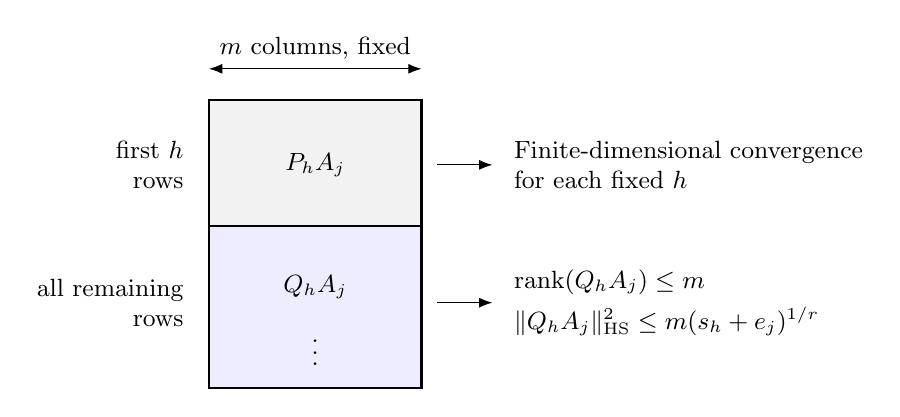
\begin{tikzpicture}[font=\small,>=Latex]
  \fill[black!5] (0,2.05) rectangle (2.7,3.65);
  \fill[blue!7] (0,0) rectangle (2.7,2.05);
  \draw[thick] (0,0) rectangle (2.7,3.65);
  \draw[thick] (0,2.05)--(2.7,2.05);
  \draw[<->] (0,4.05)--node[above]{$m$ columns, fixed}(2.7,4.05);
  \node at (1.35,2.83) {$P_hA_j$};
  \node at (1.35,1.28) {$Q_hA_j$};
  \node at (1.35,0.55) {$\vdots$};
  \node[anchor=east,align=right] at (-0.2,2.83)
       {first $h$\\rows};
  \node[anchor=east,align=right] at (-0.2,1.08)
       {all remaining\\rows};
  \draw[->] (2.9,2.83)--(3.6,2.83);
  \node[anchor=west,align=left] at (3.75,2.83)
       {Finite-dimensional convergence\\for each fixed $h$};
  \draw[->] (2.9,1.08)--(3.6,1.08);
  \node[anchor=west,align=left] at (3.75,1.08)
       {$\operatorname{rank}(Q_hA_j)\leq m$\\[4pt]
        $\|Q_hA_j\|_{\HS}^2\leq m(s_h+e_j)^{1/r}$};
 \end{tikzpicture}
 \caption{The number of rows can grow with the number of negative
 eigenfunctions, but the number of physical channels remains $m$.
 After fixing the first $h$ rows, the identity
 $K_j^2\approx B_j^2+(A_jA_j^T)^r$ bounds the operator norm in the
 remaining rows.  The rank bound converts it into a Hilbert--Schmidt
 bound, which tends to zero as first $j\to\infty$ and then $h\to\infty$.
 The drawing is schematic; all matrices are padded by zero rows in
 $\mathscr H$.}
 \label{comp:tail-figure}
\end{figure}

For each fixed $h$, the first $h$ rows of $A_j$ converge by
\eqref{comp:row-convergence}.  The first bound in
\eqref{comp:tail-bounds} makes the remaining rows uniformly small by
choosing $h$ large and then $j$ sufficiently large.  Thus $A_j$ is Cauchy in
Hilbert--Schmidt norm and converges to an operator $A:\R^m\to\mathscr H$
whose rows are precisely $a_i(x)$:
\begin{equation}
 A_j\longrightarrow A\quad\text{in Hilbert--Schmidt norm.}
 \label{comp:HS-limit}
\end{equation}
This argument applies to the whole subsequence already selected and
does not require a further choice depending on $x$.

For $B_j$ we need only pointwise compactness.  Its finite compressions
$P_hB_jP_h$ are bounded in finite-dimensional spaces, so a diagonal
subsequence makes them converge for every $h$.  Self-adjointness and
the second estimate in \eqref{comp:tail-bounds} give
\[
 \|B_j-P_hB_jP_h\|_{\op}
   \leq2\|B_jQ_h\|_{\op}
   \leq2(s_h+e_j)^{1/2}.
\]
The chosen subsequence consequently converges in operator norm to a
self-adjoint $B$ with $\|B\|_{\op}\leq\kappa$.  This subsequence, and
hence $B$, may depend on the point $x$.

We can now pass to all the required products.  Hilbert--Schmidt
convergence of $A_j$ implies operator norm convergence of
$A_jA_j^T$ and of $A_j^TA_j$.  Continuous functional calculus for
nonnegative operators then gives convergence of their $r$th powers.
Together with \eqref{comp:diagonal-limit} and
\eqref{comp:pointwise-algebra-error}, this proves
\[
 [B,\Lambda^2]=0,\qquad
 \Lambda^2-B^2=(AA^T)^r.
\]
Also $B_jA_j\to BA$ in Hilbert--Schmidt norm.  Taking its $i$th row
and using both the derivative convergence and the first-order error
in \eqref{comp:pointwise-errors} gives
$a_i'(x)=(BA)_{i,\cdot}$ for every $i$.  Finally, continuity of the
finite-dimensional Young deficit and
$Y(W,A_j^TA_j)\to0$ yield
$Y(W,A^TA)=0$.  Lemma~\ref{pre:young} gives
$W=q(A^TA)^r$.

We have proved these statements at every point of one common set of
full measure.  The construction selects no function $x\mapsto B(x)$:
only the existence of a suitable operator at each such point enters
the next section.  This completes the proof of
Proposition~\ref{comp:relations}.

\section{Fixed channels and the equality profiles}
\label{rig:section}

The pointwise relations of Proposition~\ref{comp:relations} still involve
an auxiliary operator $B$ that may depend on the point without a prescribed
measurable choice.  We now extract constant subspaces from those relations.
On each nonzero subspace, $B$ becomes a uniquely determined matrix and
satisfies an ordinary differential equation.  This will identify every
real equality potential; realification and a scalar calculation will then
complete the proof of Theorem~\ref{thm:main}.

\subsection{The channel subspaces are constant}

Assume first that $W$ is real and is a nonzero equality potential.  Use the
rows $a_i$, numbers $k_i$, and operator $\Lambda=\operatorname{diag}(k_i)$
from Proposition~\ref{comp:relations}.  For each distinct value $\alpha>0$
in the list $(k_i)$, let $n_\alpha$ be its finite multiplicity, and let
$G_\alpha$ be the $n_\alpha\times m$ matrix whose rows are the $a_i$ with
$k_i=\alpha$.  Each $G_\alpha$ has entries in $H^1(\R)$, and we use their
continuous representatives.

At every point in the common full-measure set of that proposition, choose
one of the operators $B$ it supplies.  Since $B$ commutes with $\Lambda^2$,
it preserves each of its eigenspaces.  Moreover,
\[
 AA^T=(\Lambda^2-B^2)^{1/r}
\]
commutes with both $B$ and $\Lambda^2$.  Writing $B_\alpha$ for the block
on the $\alpha^2$-eigenspace therefore gives
\begin{align}
 G_\alpha G_\beta^T&=0 &&(\alpha\ne\beta),
 \label{rig:orthogonal-blocks}\\
 G_\alpha'&=B_\alpha G_\alpha,
 & [B_\alpha,G_\alpha G_\alpha^T]&=0,
 \label{rig:block-first-order}\\
 \alpha^2I-B_\alpha^2&=(G_\alpha G_\alpha^T)^r,
 &\|B_\alpha\|_{\op}&\le\kappa.
 \label{rig:block-square}
\end{align}
These statements hold almost everywhere and require no compatibility
between the choices of $B$ at different points.

\begin{lemma}\label{rig:fixed-right-spaces}
For every $\alpha$, the subspace
\[
 \mathcal R_\alpha=(\ker G_\alpha(x))^\perp\subset\R^m
\]
is independent of $x\in\R$.  The nonzero spaces $\mathcal R_\alpha$ are
mutually orthogonal, and
\begin{equation}\label{rig:dimension-bound}
 \sum_\alpha\dim\mathcal R_\alpha\le m.
\end{equation}
In particular, only finitely many $G_\alpha$ are nonzero.  The potential
$W$ has a continuous representative, equal to zero on the orthogonal
complement of these spaces and equal to
$q(G_\alpha^TG_\alpha)^r$ on $\mathcal R_\alpha$.  With this
representative, every $G_\alpha$ is $C^2$.
\end{lemma}

\begin{proof}
Fix $v\in\R^m$.  Equation~\eqref{rig:block-first-order} implies
\[
 \|(G_\alpha v)'(x)\|\le\kappa\|G_\alpha(x)v\|
 \quad\text{for almost every }x.
\]
The function $G_\alpha v$ is locally absolutely continuous.  If it
vanishes at $x_0$, integration and Gronwall's inequality, first to the
right and then to the left of $x_0$, show that it vanishes everywhere.
Consequently $\ker G_\alpha(x)$ is independent of $x$, including points
outside the original full-measure set.  This proves the first assertion.

The products in \eqref{rig:orthogonal-blocks} are continuous, so their
almost-everywhere vanishing implies their vanishing everywhere.  Thus the
constant row spaces $\mathcal R_\alpha$ are mutually orthogonal.  Any
finite collection has total dimension at most $m$, proving
\eqref{rig:dimension-bound} and finiteness of the nonzero blocks.

On the full-measure set from Proposition~\ref{comp:relations},
$A^TA=\sum_\alpha G_\alpha^TG_\alpha$.  Each summand acts on its own
orthogonal space $\mathcal R_\alpha$, and only finitely many summands
are nonzero.  Equation~\eqref{comp:potential-limit} therefore yields
\begin{equation}\label{rig:continuous-potential}
 W=q\sum_\alpha(G_\alpha^TG_\alpha)^r
 \quad\text{almost everywhere}.
\end{equation}
The right-hand side is continuous and has the asserted restrictions;
we henceforth use it as the representative of $W$.  The row eigenfunction
equation \eqref{comp:row-eigenfunction} now reads
\begin{equation}\label{rig:block-second-order}
 G_\alpha''=\alpha^2G_\alpha-G_\alpha W
 \quad\text{in distributions}.
\end{equation}
Its right-hand side is continuous.  Integrating this identity twice shows
that the continuous representative of $G_\alpha$ is $C^2$.
\end{proof}

The row spaces already split the physical space $\R^m$ into finitely
many constant channels.  To determine the potential within one of them,
we also need a constant range for $G_\alpha$ in the eigenfunction index
space $\R^{n_\alpha}$.

\begin{lemma}\label{rig:fixed-left-spaces}
For each $\alpha$ with $\ell:=\dim\mathcal R_\alpha>0$, the range of
$G_\alpha(x)$ in $\R^{n_\alpha}$ is independent of $x$.  In constant
orthonormal bases of this range and of $\mathcal R_\alpha$, the
restriction of $G_\alpha$ is an invertible $C^2$ matrix
$D:\R\to\R^{\ell\times\ell}$.  The matrix
$B_0=D'D^{-1}$ is $C^1$ and satisfies, everywhere on $\R$,
\begin{equation}\label{rig:active-identities}
 B_0=B_0^T,\qquad
 \alpha^2I-B_0^2=(DD^T)^r>0,\qquad
 B_0'=r(B_0^2-\alpha^2I).
\end{equation}
\end{lemma}

\begin{proof}
Choose a constant orthonormal basis of $\mathcal R_\alpha$, and let
$E(x)$ be the matrix of the restriction of $G_\alpha(x)$ to this space.
It has full column rank $\ell$ at every point, since the kernel of
$G_\alpha$ is constant.  The projection onto its range is
\[
 P(x)=E(x)(E(x)^TE(x))^{-1}E(x)^T.
\]
The commutator in \eqref{rig:block-first-order} shows that $B_\alpha$
preserves the range of $G_\alpha G_\alpha^T$, which is precisely the
range of $E$.  Hence $E'=B_\alpha E$ has its columns in this range
almost everywhere.  Differentiating the projection gives
\begin{align*}
 P'={}&(I-P)E'(E^TE)^{-1}E^T\\
     &+E(E^TE)^{-1}(E')^T(I-P)=0
 \quad\text{almost everywhere}.
\end{align*}
Since $P$ is $C^1$, it is constant.

Choose a constant orthonormal basis of this range as well.  The resulting
square matrix $D$ is invertible everywhere and $C^2$.  Almost everywhere,
$D'D^{-1}$ is the restriction of $B_\alpha$ to its invariant range in
these coordinates.  Equations~\eqref{rig:block-first-order} and
\eqref{rig:block-square} give the symmetry and square identity in
\eqref{rig:active-identities} almost everywhere; continuity extends
them to every point.  Positivity is strict because $D$ is invertible.

On $\mathcal R_\alpha$, Equation~\eqref{rig:continuous-potential}
identifies the potential with $q(D^TD)^r$.  Equation~
\eqref{rig:block-second-order} consequently becomes
\[
 D''=\alpha^2D-qD(D^TD)^r
     =\alpha^2D-q(DD^T)^rD.
\]
The second equality follows, for example, by a singular-value
decomposition.  Differentiating $B_0=D'D^{-1}$ and using $q=r+1$
now gives
\[
 B_0'=D''D^{-1}-B_0^2
      =\alpha^2I-q(\alpha^2I-B_0^2)-B_0^2
      =r(B_0^2-\alpha^2I),
\]
as claimed.
\end{proof}

\subsection{The matrix Riccati equation separates the profiles}

Fix a nonzero block and the matrices of Lemma~\ref{rig:fixed-left-spaces}.
Diagonalize the symmetric matrix $B_0(x_*)$ at one point by a constant
orthogonal change of range coordinates.  The right-hand side of its
Riccati equation is a polynomial in $B_0$.  Uniqueness for this matrix
ordinary differential equation therefore preserves the diagonal form.
More explicitly, the strict inequality in \eqref{rig:active-identities}
places each initial diagonal entry in $(-\alpha,\alpha)$.  There is a
unique $y_j\in\R$ such that the scalar solution with that initial value is
\begin{equation}\label{rig:tanh}
 b_j(x)=-\alpha\tanh\bigl(r\alpha(x-y_j)\bigr),
 \qquad 1\le j\le\ell.
\end{equation}
The diagonal matrix with these entries solves the same initial-value
problem as $B_0$ on all of $\R$, so uniqueness gives equality everywhere.

Equation~\eqref{rig:active-identities} implies that $DD^T$ is diagonal
in these coordinates.  Since $D'=\operatorname{diag}(b_j)D$, each row
of $D$ is a positive scalar multiple of its value at $x_*$.  None of
these rows is zero, and their directions are mutually orthogonal because
$DD^T$ is diagonal.  Taking their normalized directions as a constant
orthonormal basis of $\mathcal R_\alpha$ makes $D$ diagonal with positive
entries.  The potential in this fixed basis is therefore diagonal, with
entries
\begin{equation}\label{rig:profiles}
 q\bigl(\alpha^2-b_j(x)^2\bigr)
 =(r+1)\alpha^2\operatorname{sech}^2\bigl(r\alpha(x-y_j)\bigr).
\end{equation}
Combining these bases over the finitely many nonzero spaces
$\mathcal R_\alpha$, and adding a basis of their orthogonal complement,
proves the required necessity for real $W$.  There are at most $m$
nonzero profiles by \eqref{rig:dimension-bound}.  The zero potential
has the same description with no nonzero profile.

\subsection{Complex Hermitian potentials}

For a complex Hermitian potential $W$, take the realification
$\widetilde W$ from \eqref{bound:realification}.  The proof of
Proposition~\ref{bound:sharp} shows that it is equivalent to
$W\oplus\overline W$ by a constant unitary matrix and that both the trace-power
integral and the negative spectral moment are doubled.  Thus equality
for $W$ implies equality for the real potential $\widetilde W$.

The real result provides a constant unitary matrix $V$ such that
\[
 W(x)\oplus\overline W(x)
   =V\operatorname{diag}(f_1(x),\ldots,f_{2m}(x))V^*
 \quad\text{almost everywhere},
\]
where each $f_j$ is either a profile of the form \eqref{rig:profiles} or
zero.  Let $P$ be the projection onto the first summand $\C^m$ and put
$\widehat P=V^*PV$.  Since $P$ commutes with $W\oplus\overline W$,
\[
 (f_i(x)-f_j(x))\widehat P_{ij}=0
 \quad\text{almost everywhere}.
\]
Consequently $\widehat P_{ij}=0$ whenever the functions $f_i,f_j$ are
not equal almost everywhere.  Partition the indices into groups of
identical functions, including the possible zero function.  The range
of $\widehat P$ splits as the orthogonal sum of its intersections with
these coordinate groups.  On each group the diagonal potential is a
scalar multiple of the identity, so any constant orthonormal basis of
that intersection diagonalizes its restriction.  Transporting these
bases by $V$ to the first summand gives a constant unitary basis of
$\C^m$ in which $W$ has the asserted profiles.  This proves necessity
for complex Hermitian potentials.

\subsection{Each listed potential attains equality}

It remains to verify attainment, including the exact spectral moment,
without appealing to a classification of scalar optimizers.  Fix $a>0$
and $x_0\in\R$, and set
\[
 V(x)=(r+1)a^2\operatorname{sech}^2\bigl(ra(x-x_0)\bigr),
 \qquad H=-\partial_x^2-V.
\]
The first-order factorization used in the commutation argument
of~\cite[Section~II]{BenguriaLoss2000} also explains why this profile has
only one negative eigenvalue.  Put
\[
 w(x)=a\tanh\bigl(ra(x-x_0)\bigr),
 \qquad Q=\partial_x+w,\qquad \operatorname{Dom}Q=H^1(\R).
\]
Then $Q^*=-\partial_x+w$ on $H^1(\R)$.  Since $w$ and $w'$ are bounded,
both product domains are $H^2(\R)$, and direct differentiation yields
\begin{align}
 Q^*Q&=H+a^2,
 \label{rig:factorization}\\
 QQ^*&=-\partial_x^2+a^2
       +(r-1)a^2\operatorname{sech}^2\bigl(ra(x-x_0)\bigr)
       \ge a^2.
 \label{rig:partner}
\end{align}
Here the last inequality uses $r>1$.  The equation $Q\psi=0$ has the
one-dimensional $L^2$ solution space
\[
 \ker Q=
 \operatorname{span}\left\{
    \operatorname{sech}^{1/r}\bigl(ra(x-x_0)\bigr)
 \right\}.
\]
Thus $-a^2$ is a simple eigenvalue of $H$, and
\eqref{rig:factorization} excludes eigenvalues below it.  If
$H\phi=\lambda\phi$ with $-a^2<\lambda<0$, put
$\mu=\lambda+a^2$ and $g=Q\phi$.  Then
$\|g\|_2^2=\mu\|\phi\|_2^2>0$.  Moreover,
$Q^*Q\phi=\mu\phi\in\operatorname{Dom}Q$, so
$g\in\operatorname{Dom}(QQ^*)$ and $QQ^*g=\mu g$.  This contradicts
\eqref{rig:partner}, since $\mu<a^2$.  By Lemma~\ref{pre:spectral},
all negative spectrum is discrete.  Hence $-a^2$ is the sole negative
eigenvalue.

Finally, $2p-1=2\gamma$ and the substitution $s=\tanh y$ give
\begin{align*}
 \int_\R V(x)^p\,dx
 &=\frac{(r+1)^p}{r}a^{2\gamma}
     \int_\R\operatorname{sech}^{2p}y\,dy\\
 &=\frac{(r+1)^p}{r}a^{2\gamma}
     \int_{-1}^{1}(1-s^2)^{p-1}\,ds
  =\frac{b_\sigma}{D_\sigma}a^{2\gamma},
\end{align*}
where $(r+1)^p/r=D_\sigma^{-1}$ and $p-1=\sigma$.  Consequently
\[
 \operatorname{Tr}(H)_-^\gamma
   =a^{2\gamma}
   =C_\gamma\int_\R V^p.
\]
The zero potential contributes zero to both sides.  Finite orthogonal
direct sums add the spectral moments and trace-power integrals, and a
constant unitary conjugation leaves both unchanged.  Every potential
listed in Theorem~\ref{thm:main} therefore attains equality, completing
its proof.

\appendix
\section{The exact integrated trace deficit}\label{app:trace}

The matrix comparison needed in the action argument has an exact
remainder.  We give the proof from \cite[Section~3]{MLT}, retaining
both nonnegative terms.  Together they control the commutator and
the algebraic equality relation used in the action argument.
Throughout this appendix, $0<\sigma<1$, $\beta=\sigma-\tfrac12$, and
$r=1/\sigma$, $p=1+\sigma$, $q=1+r$.
Define $c_\sigma>0$ by
\begin{equation}\label{trace:normalization}
 c_\sigma^{-1}
 =\int_0^\infty t^\beta
       \bigl(t^{-1/2}-(t+1)^{-1/2}\bigr)\,dt.
\end{equation}
The integrand is $O(t^{\sigma-1})$ at zero and
$O(t^{\sigma-2})$ at infinity.  Scaling therefore gives
\begin{equation}\label{trace:scaling}
 c_\sigma\int_0^\infty t^\beta
       \bigl(t^{-1/2}-(t+y)^{-1/2}\bigr)\,dt=y^\sigma,
 \qquad y\geq0.
\end{equation}

\begin{theorem}[Exact trace deficit]\label{trace:deficit}
Let $n\geq1$ and let $B,V\in\C^{n\times n}$ be Hermitian.
Suppose that
\begin{equation}\label{trace:symbol}
 Y_s=(sI-B)^2,\qquad X_s=Y_s+V\geq bI
 \quad(s\in\R)
\end{equation}
for some $b>0$.  Set
\begin{equation}\label{trace:resolvents}
 R(t)=\frac1\pi\int_\R(X_s+tI)^{-1}\,ds,
 \qquad P(t)=t^{-1/2}I-R(t),\qquad t>0,
\end{equation}
and
\begin{equation}\label{trace:N}
 N=c_\sigma\int_0^\infty t^\beta P(t)\,dt.
\end{equation}
These integrals converge absolutely in matrix norm, and $R(t)>0$.
There are continuous Hermitian matrices $L(t)=R(t)^{-1}>0$ and
$Z(t)$ satisfying
\begin{equation}\label{trace:LZ}
 V+tI=L^2+Z^2+i[B,Z],\qquad
 LZ+ZL+i[B,L]=0.
\end{equation}
If $N\geq0$, then
\begin{equation}\label{trace:deficit-identity}
 \begin{split}
 \tr(NV)-\tr(N^q)
 =c_\sigma\int_0^\infty t^\beta\Bigl(
    \tr(RZ^2)
    +q\bigl\|R^{-1/2}-R^{1/2}(tI+N^r)^{1/2}\bigr\|_{\HS}^2
    \Bigr)\,dt.
 \end{split}
\end{equation}
In particular, $\tr(NV)\geq\tr(N^q)$.
\end{theorem}

The hypothesis concerns the full symbol $X_s$; the perturbation
$V$ itself need not be positive.  The proof first recovers $L$ and
$Z$ from solutions on the two half-lines, then evaluates a logarithmic
integral, and finally completes a matrix square.

\subsection{Half-line boundary maps}

Quadratic growth in $s$, together with \eqref{trace:symbol}, gives
an integrable bound for $X_s^{-1}$.  Hence $R(t)>0$ and
$R(t)=O(1)$ as $t\downarrow0$.  Diagonalization of $B$ gives
\[
 \frac1\pi\int_\R(Y_s+tI)^{-1}\,ds=t^{-1/2}I.
\]
For $t\geq1$, both $X_s+tI$ and $Y_s+tI$ dominate
$c(s^2+t)I$, with $c>0$ independent of $s,t$.
The resolvent identity bounds their inverse difference by
$C(s^2+t)^{-2}$, and therefore
\begin{equation}\label{trace:P-bounds}
 \|P(t)\|_{\op}=
 \begin{cases}
  O(t^{-1/2}),&t\downarrow0,\\
  O(t^{-3/2}),&t\to\infty.
 \end{cases}
\end{equation}
These bounds prove the asserted convergence of $N$.

Fix $t>0$ and put $\nabla=\partial_x-iB$.  We shall use the
equation
\begin{equation}\label{trace:ode}
 (-\nabla^2+V+tI)\psi=0.
\end{equation}
Matrix Riccati equations also appear in the commutation method for
Schr\"odinger inequalities \cite{BenguriaLoss2000}.  Here their role
is to compute the integrated resolvent through boundary data.

For each $v\in\C^n$ there is a unique $H^1$ solution of
\eqref{trace:ode} on either half-line with $\psi(0)=v$.
Indeed, the sesquilinear form
\[
 a_t(\phi,\psi)=\int
  \bigl(\langle\nabla\phi,\nabla\psi\rangle
       +\langle\phi,(V+tI)\psi\rangle\bigr)\,dx,
\]
with inner products linear in the second variable, is coercive on
$H^1(\R;\C^n)$: its Fourier symbol $X_s+tI$ dominates
$c_t(1+s^2)I$.  Zero extension gives coercivity on the trace-zero
subspace of either half-line.  Correcting any $H^1$ extension of
$v$ by the Riesz representation theorem gives the unique weak
solution.  The equation implies $\psi''\in L^2$, so this solution
lies in $H^2$; both $\psi$ and $\psi'$ vanish at the infinite end.

Define the right and left boundary matrices $S,T$ by
\begin{equation}\label{trace:boundary}
 \nabla\psi(0+)=-Sv,\qquad \nabla\psi(0-)=Tv.
\end{equation}
Integration by parts gives
$a_t(\psi_v,\psi_w)=\langle v,Sw\rangle$ on the right and
$a_t(\psi_v,\psi_w)=\langle v,Tw\rangle$ on the left.  Thus
$S,T$ are Hermitian.  Translation and uniqueness show that
$\nabla\psi=-S\psi$ throughout the right half-line and
$\nabla\psi=T\psi$ throughout the left half-line.
Substituting these relations into \eqref{trace:ode}, and allowing
arbitrary boundary data, gives
\begin{equation}\label{trace:riccati}
 V+tI=S^2+i[B,S]=T^2-i[B,T].
\end{equation}

Glue the two solutions with boundary value $v$ at zero.
The resulting continuous function has derivative jump
$-(S+T)v$, and hence satisfies
\[
 (-\nabla^2+V+tI)\psi=\delta_0(S+T)v.
\]
Fourier inversion, with forward kernel $e^{-isx}$, gives
\[
 v=\frac1{2\pi}\int_\R(X_s+tI)^{-1}\,ds\,(S+T)v
   =\tfrac12 R(t)(S+T)v.
\]
The inverse symbol is $O(s^{-2})$, so its Fourier inverse is
continuous and this evaluation at zero is justified.  Therefore
\[
 L:=\tfrac12(S+T)=R^{-1}>0,\qquad Z:=\tfrac12(S-T)
\]
satisfy \eqref{trace:LZ}, by adding and subtracting
\eqref{trace:riccati}.  The second equation in \eqref{trace:LZ}
determines $Z$ uniquely from $L$, since $L>0$; in an eigenbasis
of $L$, the map $Z\mapsto LZ+ZL$ multiplies its $(j,k)$ entry
by the positive number $L_{jj}+L_{kk}$.  This also proves the
continuity of $Z(t)$, because $R(t)$, and hence $L(t)$, is continuous.

The diagonal entries of that same equation give $Z_{jj}=0$
in an eigenbasis of $L$, so $\tr Z=0$.  Multiplication on both
sides by $R=L^{-1}$ gives
$i[R,B]=-(ZR+RZ)$.  Cyclicity of the trace now yields
\begin{equation}\label{trace:RV}
 \tr\bigl(R(V+tI)\bigr)=\tr L-\tr(RZ^2).
\end{equation}
In particular, the correction $\tr(RZ^2)=\tr(ZRZ)$ is nonnegative.
We will also need the location of the spectrum of $B+iS$.
The right solutions obey $\psi'=i(B+iS)\psi$.
For an eigenvector with eigenvalue $z$, the solution is $e^{izx}v$;
its square integrability forces $\operatorname{Im}z>0$.

\subsection{A logarithmic integral}

The next step converts the boundary matrices into a scalar identity
that can be integrated in $t$.  Define
\begin{equation}\label{trace:F}
 F(t)=\frac{\tr V}{\sqrt t}
       -\frac1\pi\int_\R
          \log\frac{\det(X_s+tI)}{\det(Y_s+tI)}\,ds.
\end{equation}
The determinants are positive, and the logarithmic ratio is
$O(|s|^{-2})$ at infinity.  Its derivative in $t$ is the trace
of the resolvent difference, with an integrable bound locally
uniform for $t>0$.  Thus the integral converges absolutely and
$F$ is continuously differentiable.

The first identity in \eqref{trace:riccati} factors the symbol as
\[
 X_s+tI=(sI-B+iS)(sI-B-iS).
\]
If $u_j+iv_j$ are the eigenvalues of $B+iS$, counted with
algebraic multiplicity, then $v_j>0$ and
\[
 \det(X_s+tI)=\prod_{j=1}^n\bigl((s-u_j)^2+v_j^2\bigr).
\]
The denominator in \eqref{trace:F} has the same form, with centers
the eigenvalues of $B$ and widths $\sqrt t$.
Translations of the individual logarithms change their
symmetric-cutoff integrals by $o(1)$: for
$h(s)=\log(s^2+v^2)$,
\[
 \frac{d}{da}\int_{-M}^M h(s-a)\,ds
       =h(M+a)-h(M-a)\longrightarrow0
\]
uniformly for bounded $a$.  After centering the factors, the identity
\[
 \int_\R\log\frac{s^2+v^2}{s^2+w^2}\,ds=2\pi(v-w),
 \qquad v,w>0,
\]
follows by differentiation in $v$ and integration from $w$ to $v$.
Since $\sum_jv_j=\tr S=\tr L$, we obtain
\begin{equation}\label{trace:F-evaluation}
 F(t)=\frac{\tr V}{\sqrt t}-2\tr(L-\sqrt t I).
\end{equation}

Set
\begin{equation}\label{trace:G}
 G(t)=\tr(L-2\sqrt t I+tR).
\end{equation}
Both functions are nonnegative.  For $G$, apply
$\lambda-2\sqrt t+t/\lambda\geq0$ to the positive eigenvalues
$\lambda$ of $L$.  For $F$, take the trace of \eqref{trace:LZ}
and use \eqref{trace:F-evaluation} to obtain
\[
 F(t)=t^{-1/2}\tr\bigl((L-\sqrt t I)^2+Z^2\bigr)\geq0.
\]
Equations \eqref{trace:RV} and \eqref{trace:F-evaluation} give
the identity
\begin{equation}\label{trace:FG}
 \tr(PV)=F+G+\tr(RZ^2).
\end{equation}
Every term on the right is nonnegative.  The bounds
\eqref{trace:P-bounds} therefore show that $F$, $G$, and
$\tr(RZ^2)$ are integrable against $t^\beta\,dt$, and that
$t^{\beta+1}F(t)$ vanishes at both endpoints.

Differentiating \eqref{trace:F} and using
\eqref{trace:F-evaluation}--\eqref{trace:G} gives
\[
 F'(t)=-\frac{\tr V}{2t^{3/2}}+\tr P(t),
 \qquad tF'(t)=-\tfrac12F(t)-G(t).
\]
Integration by parts, with the endpoint limits just proved, yields
$\int_0^\infty t^\beta G\,dt
 =\sigma\int_0^\infty t^\beta F\,dt$.
Consequently, integration of \eqref{trace:FG} gives
\begin{equation}\label{trace:weighted}
 \tr(NV)=q c_\sigma\int_0^\infty t^\beta G(t)\,dt
       +c_\sigma\int_0^\infty t^\beta\tr(RZ^2)\,dt.
\end{equation}
It remains to express the first integral as $\tr(N^q)/q$ plus
a nonnegative remainder.

\subsection{The noncommutative square}

For a positive semidefinite matrix $D$, let
\[
 F_0(t,D)=\frac{\tr D}{\sqrt t}
       -2\tr\bigl((tI+D)^{1/2}-\sqrt t I\bigr).
\]
For a scalar eigenvalue $d\geq0$, the corresponding summand is
$\int_0^d(t^{-1/2}-(t+y)^{-1/2})\,dy$.
Tonelli's theorem and \eqref{trace:scaling} therefore imply
\begin{equation}\label{trace:F0}
 c_\sigma\int_0^\infty t^\beta F_0(t,D)\,dt
     =\frac1p\tr(D^p).
\end{equation}
Now expand the Hilbert--Schmidt square
\begin{align}
 \mathcal D_D(t)
  &:=\bigl\|R^{-1/2}-R^{1/2}(tI+D)^{1/2}\bigr\|_{\HS}^2
       \notag\\
  &=\tr\bigl(R^{-1}+R(tI+D)-2(tI+D)^{1/2}\bigr)
       \label{trace:square}\\
  &=G(t)-\tr(P(t)D)+F_0(t,D).\notag
\end{align}
No commutation is used: the cross terms cancel adjacent factors
$R^{-1/2}R^{1/2}$, and cyclicity changes the remaining quadratic
term into $\tr(R(tI+D))$.
All three terms in the last line are integrable by
\eqref{trace:P-bounds}, \eqref{trace:FG}, and \eqref{trace:F0}.
Thus
\begin{equation}\label{trace:duality}
 c_\sigma\int_0^\infty t^\beta G(t)\,dt
  =\tr(ND)-\frac1p\tr(D^p)
       +c_\sigma\int_0^\infty t^\beta\mathcal D_D(t)\,dt.
\end{equation}
When $N\geq0$, choose $D=N^r$.  Since $rp=q=1+r$,
the first two terms on the right equal $\tr(N^q)/q$.
Substitution into \eqref{trace:weighted} proves
\eqref{trace:deficit-identity} and completes the proof of
Theorem~\ref{trace:deficit}.

If $B$ and $V$ commute, the symbol hypothesis implies $V\geq bI$.
Simultaneous diagonalization then gives
$R(t)=(tI+V)^{-1/2}$, $N=V^\sigma$, and $Z=0$.
Both remainders vanish, as required by scalar equality.

\section{The regularized field and connecting paths}
\label{app:paths}

The finite-interval action argument requires a symmetric matrix path
from $K$ to $-K$ whose derivative measures the difference between a
matrix field and $AA^{\mathsf T}$.  We construct both the field and the
path here.  These are the constructions of \cite[Sections~4--5]{MLT};
we include their proofs to make the analytic input to the equality
argument self-contained.  The positivity statement below also
identifies the resolvent to which Theorem~\ref{trace:deficit} applies.

Throughout this appendix,
$K=\operatorname{diag}(k_1,\ldots,k_n)$ with $k_i>0$,
$\kappa=\max_i k_i$, and $\Sym_n$ denotes the real symmetric matrices.
We use $\beta=\sigma-\tfrac12$ and the constant $c_\sigma$ from
\eqref{trace:normalization}.

\subsection{A field with a scalar boundary integral}

For $\delta>0$, define on $y\geq0$
\begin{equation}\label{field:f}
 f_\delta(y)=\frac{c_\sigma}{\pi}\int_0^\infty t^\beta
       \left(\frac1{t+\delta}-\frac1{t+\delta+y}\right)\,dt,
\end{equation}
and extend to $y<0$ by the tangent line $f_\delta'(0)y$.
The resulting function is $C^1$, strictly increasing, and concave.
Indeed, for $y\geq0$,
\begin{equation}\label{field:f-derivative}
 f_\delta'(y)=a_\sigma(y+\delta)^{\beta-1},
 \qquad
 a_\sigma=\frac{c_\sigma}{\pi}
       \int_0^\infty\frac{u^\beta}{(1+u)^2}\,du>0.
\end{equation}
Both integrals converge since $-\tfrac12<\beta<\tfrac12$.
The extension allows the functional calculus below even when its
matrix argument has negative eigenvalues.

Set
\begin{equation}\label{field:definition}
 \begin{split}
 Q_s(B)&=s^2I-2sB+K^2,\\
 M_\delta(B)&=\lim_{R\to\infty}\int_{-R}^{R}
       \bigl(f_\delta(Q_s(B))-f_\delta(s^2)I\bigr)\,ds,
       \qquad B\in\Sym_n,
 \end{split}
\end{equation}
where the symmetric cutoff cancels the leading term
$-2s f_\delta'(s^2)B$, which is odd in $s$.
The scalar counterpart is
\begin{equation}\label{field:mu}
 \mu_\delta(z)=\int_\R
     \bigl(f_\delta(s^2+z)-f_\delta(s^2)\bigr)\,ds,
       \qquad z\in\R.
\end{equation}

\begin{proposition}[Regularized field]\label{field:properties}
The limit in \eqref{field:definition} exists locally uniformly, and
$M_\delta:\Sym_n\to\Sym_n$ is locally Lipschitz.  There is a
$C^1$ function $J_\delta:\Sym_n\to\R$, normalized by
$J_\delta(0)=0$, such that
\begin{equation}\label{field:primitive}
 dJ_\delta(B)[H]=-\tr(M_\delta(B)H).
\end{equation}
The scalar function $\mu_\delta$ is locally Lipschitz and strictly
increasing, with $\mu_\delta(0)=0$, and
\begin{equation}\label{field:mu-positive}
       \mu_\delta(z)=(z+\delta)^\sigma-\delta^\sigma
       \qquad(z\geq0).
\end{equation}
For every real unit vector $e$, and for every standard basis vector
$e_i$, respectively,
\begin{align}
 e^{\mathsf T}M_\delta(B)e
  &\leq\mu_\delta\bigl(e^{\mathsf T}K^2e
                         -(e^{\mathsf T}Be)^2\bigr),
       \label{field:direction}\\
 Be_i=ye_i\quad&\Longrightarrow\quad
 M_\delta(B)e_i=\mu_\delta(k_i^2-y^2)e_i.
       \label{field:coordinate}
\end{align}
For each diagonal sign matrix $S$,
\begin{equation}\label{field:equivariance}
                 M_\delta(SBS)=SM_\delta(B)S.
\end{equation}
Finally,
\begin{equation}\label{field:endpoints}
 \begin{split}
 J_\delta(-K)-J_\delta(K)
 &=\sum_{i=1}^n\int_{-k_i}^{k_i}\mu_\delta(k_i^2-s^2)\,ds\\
 &\longrightarrow b_\sigma\sum_{i=1}^n k_i^{2\sigma+1}
       \qquad(\delta\downarrow0).
 \end{split}
\end{equation}
\end{proposition}

\begin{proof}
We first justify the matrix integral, including its local Lipschitz
dependence.  If a scalar function $h$ is Lipschitz on an interval
containing the spectra of Hermitian matrices $X,Y$, then
\begin{equation}\label{field:HS-calculus}
 \|h(X)-h(Y)\|_{\HS}\leq\operatorname{Lip}(h)\|X-Y\|_{\HS}.
\end{equation}
To see this, use eigenbases $e_i$ of $X$ and $v_j$ of $Y$.
The mixed matrix entries of the two differences are
$(h(\lambda_i)-h(\nu_j))\langle e_i,v_j\rangle$ and
$(\lambda_i-\nu_j)\langle e_i,v_j\rangle$; square the scalar
Lipschitz inequality and sum over $i,j$.

On a bounded set of $B$'s the spectrum of
$E_s(B)=-2sB+K^2$ is contained in $[-a|s|,a|s|]$ for all sufficiently
large $|s|$.  For
\[
 h_s(y)=f_\delta(s^2+y)-f_\delta(s^2)-f_\delta'(s^2)y,
\]
Equation~\eqref{field:f-derivative} gives
$\sup_{|y|\leq a|s|}|h_s'(y)|=O(|s|^{2\beta-3})$.
It follows from \eqref{field:HS-calculus} that
\[
 f_\delta(Q_s(B))-f_\delta(s^2)I
      =-2s f_\delta'(s^2)B+T_s(B),
\]
where both $\|T_s(B)\|_{\HS}$ and the local Lipschitz constant of
$T_s$ are $O(|s|^{2\beta-2})$.  For the first bound, include
$f_\delta'(s^2)K^2$ in $T_s$; for the second, apply
\eqref{field:HS-calculus} to $h_s(E_s(B))$ and use
$E_s(B_1)-E_s(B_2)=-2s(B_1-B_2)$.
Because $2\beta-2<-1$, these remainders are integrable at infinity.
The odd term cancels at each symmetric cutoff.  On bounded
$s$-intervals, \eqref{field:HS-calculus} applies directly to
$f_\delta$.  This proves the asserted convergence and regularity.

For the primitive, choose a scalar antiderivative
$g_\delta'=f_\delta$.  Trace differentiation gives
$d\tr(g_\delta(X))[H]=\tr(f_\delta(X)H)$.
This formula follows for polynomials by cyclicity and for
$g_\delta$ by approximation in $C^1$ on compact spectral intervals.
For $s\ne0$, the function
\[
 B\longmapsto
 \frac{\tr(g_\delta(Q_s(B))-g_\delta(K^2))}{2s}
                  +f_\delta(s^2)\tr B
\]
has differential
$-\tr((f_\delta(Q_s(B))-f_\delta(s^2)I)H)$.
At $s=0$ that differential is constant in $B$ and also has a
primitive.  Thus the negative of every finite-cutoff field has
zero integral around each closed piecewise smooth curve in
$\Sym_n$.  Local uniform convergence passes this property to
$-M_\delta$.  Path integration, starting at zero, defines
$J_\delta$ and proves \eqref{field:primitive}.

For bounded $z$, the integrand in \eqref{field:mu} and its
Lipschitz constant in $z$ are $O(|s|^{2\beta-2})$ at infinity.
This proves absolute convergence and local Lipschitz continuity
of $\mu_\delta$.  Strict increase and $\mu_\delta(0)=0$ follow
from the same properties of $f_\delta$.  For $z\geq0$,
Tonelli's theorem applied to \eqref{field:f} gives
\[
 \mu_\delta(z)=c_\sigma\int_0^\infty t^\beta
       \bigl((t+\delta)^{-1/2}-(t+\delta+z)^{-1/2}\bigr)\,dt.
\]
The normalization \eqref{trace:normalization}, after scaling,
evaluates this as \eqref{field:mu-positive}.

Translations in the variable $s$ remain legitimate with a
symmetric cutoff.  More precisely, for fixed $a,z\in\R$,
\begin{equation}\label{field:shift}
 \lim_{R\to\infty}\int_{-R}^{R}
   \bigl(f_\delta((s-a)^2+z)-f_\delta(s^2)\bigr)\,ds
          =\mu_\delta(z).
\end{equation}
Indeed $F_z(s)=f_\delta(s^2+z)$ is even and
$F_z'(s)=O(|s|^{2\beta-1})\to0$ at infinity.  Pairing the two
short intervals produced by a translation bounds the difference
between the shifted and unshifted cutoff integrals by
\[
 |a|^2\sup_{R-|a|\leq u\leq R+|a|}|F_z'(u)|,
\]
which tends to zero.

Scalar concavity in an eigenbasis of $Q_s(B)$ now gives
\[
 e^{\mathsf T}f_\delta(Q_s(B))e
     \leq f_\delta(e^{\mathsf T}Q_s(B)e).
\]
The scalar argument on the right is
$(s-e^{\mathsf T}Be)^2+e^{\mathsf T}K^2e-(e^{\mathsf T}Be)^2$.
Integration and \eqref{field:shift} prove \eqref{field:direction}.
If $Be_i=ye_i$, functional calculus gives equality in the
corresponding coordinate, proving \eqref{field:coordinate}.
Since $SK^2S=K^2$, conjugation inside the defining integral proves
\eqref{field:equivariance}.

On diagonal matrices, \eqref{field:primitive} and
\eqref{field:coordinate} read
\[
 dJ_\delta(\operatorname{diag}(b_1,\ldots,b_n))
       =-\sum_i\mu_\delta(k_i^2-b_i^2)\,db_i.
\]
Integrating from $K$ to $-K$ gives the first equality in
\eqref{field:endpoints}.  For $z\geq0$,
$0\leq\mu_\delta(z)\leq z^\sigma$ and
$\mu_\delta(z)\to z^\sigma$.  Dominated convergence and the
substitution $s=k_i u$ give its stated limit.
\end{proof}

The field is defined on all symmetric matrices, but the action
argument compares it with a positive matrix $AA^{\mathsf T}$.
At such values its directional bound forces positivity of the
entire quadratic symbol $Q_s(B)$.  This is the condition needed
for the trace deficit formula.

\begin{proposition}[Positive values of the field]\label{field:positive}
If $M=M_\delta(B)\geq0$, then
\begin{equation}\label{field:positive-bounds}
 Q_s(B)\geq0\quad(s\in\R),\qquad
             0\leq M\leq\kappa^{2\sigma}I.
\end{equation}
Set $V=K^2-B^2+\delta I$ and use $B,V$ in
\eqref{trace:resolvents} and \eqref{trace:N}.  Then the symbol
$(sI-B)^2+V=Q_s(B)+\delta I$ is bounded below by $\delta I$, and
\begin{equation}\label{field:N}
                         N=M+\delta^\sigma I.
\end{equation}
In particular, the hypotheses of Theorem~\ref{trace:deficit} hold.
\end{proposition}

\begin{proof}
By \eqref{field:direction}, positivity of $M$ and strict increase
of $\mu_\delta$ imply
$e^{\mathsf T}K^2e\geq(e^{\mathsf T}Be)^2$ for every real unit
vector $e$.  Completing the scalar square gives
\[
 e^{\mathsf T}Q_s(B)e=(s-e^{\mathsf T}Be)^2
                +e^{\mathsf T}K^2e-(e^{\mathsf T}Be)^2\geq0.
\]
Thus $Q_s(B)\geq0$, also as a Hermitian matrix on $\C^n$.
Moreover, \eqref{field:direction} gives
$M\leq\mu_\delta(\kappa^2)I\leq\kappa^{2\sigma}I$, using
$(a+b)^\sigma\leq a^\sigma+b^\sigma$.

Write $Y_s=(sI-B)^2$.  Diagonalization of $B$ and
\eqref{field:shift} allow replacement of the scalar subtraction
$f_\delta(s^2)I$ in \eqref{field:definition} by $f_\delta(Y_s)$.
Since both $Q_s(B)$ and $Y_s$ are positive, their difference under
$f_\delta$ is, by \eqref{field:f},
\[
 \frac{c_\sigma}{\pi}\int_0^\infty t^\beta
 \left((Y_s+(t+\delta)I)^{-1}
          -(Q_s(B)+(t+\delta)I)^{-1}\right)\,dt.
\]
For fixed $B,\delta$, both matrices being inverted are bounded
below by $c(1+t+s^2)I$.  Their difference is $K^2-B^2$, so the
resolvent identity bounds the norm of the integrand by
$C t^\beta(1+t+s^2)^{-2}$.  Integrating first in $s$ yields
$C't^\beta(1+t)^{-3/2}$, which is integrable on $(0,\infty)$.
Fubini's theorem is therefore applicable and gives
\[
 M=c_\sigma\int_0^\infty t^\beta
        \bigl((t+\delta)^{-1/2}I-R(t)\bigr)\,dt.
\]
Subtracting this expression from \eqref{trace:N} and scaling
\eqref{trace:normalization} gives \eqref{field:N}.
\end{proof}

\subsection{Choosing the lower triangular coefficient matrix}

Let $\mathcal L_n$ be the real lower triangular $n\times n$
matrices.  Their dimension equals that of $\Sym_n$.  This dimension
match allows us to prescribe a symmetric terminal value by choosing
$C\in\mathcal L_n$.  At a simple initial problem there is one choice
up to signs of the rows.  Continuation preserves the parity of this
number, and hence produces the required terminal value.

\begin{proposition}[Connecting path]\label{path:connecting}
Let $\Omega=(x_-,x_+)$ be bounded and let
$U\in H^1_0(\Omega;\R^{n\times d})$, where $n,d\geq1$, satisfy
\[
                         \int_\Omega UU^{\mathsf T}\,dx=I_n.
\]
For every $\delta,\varepsilon>0$ there are
$C_\varepsilon\in\mathcal L_n$ and
$B_\varepsilon\in C^1(\overline\Omega;\Sym_n)$ such that, with
$A_\varepsilon=C_\varepsilon U$,
\begin{equation}\label{path:ode}
 \varepsilon B_\varepsilon'
       =M_\delta(B_\varepsilon)-A_\varepsilon A_\varepsilon^{\mathsf T},
 \qquad B_\varepsilon(x_-)=K,\quad B_\varepsilon(x_+)=-K.
\end{equation}
They satisfy
\begin{equation}\label{path:bounds}
 \sup_{x\in\overline\Omega}\|B_\varepsilon(x)\|_{\op}\leq\kappa,
 \qquad
 \sup_{0<\varepsilon\leq1}\|C_\varepsilon\|_{\HS}<\infty,
\end{equation}
where the second bound is for fixed $\delta,K,\Omega$.
\end{proposition}

\begin{proof}
Use the continuous representative of $U$.  Choose a smooth,
nonnegative, compactly supported cutoff $\chi$ on $\Sym_n$, equal
to one on $\{B:\|B\|_{\op}\leq\kappa\}$ and invariant under
conjugation by diagonal sign matrices.  Averaging a cutoff over
the finite sign group produces such a function.  The truncated
field $\widehat M=\chi M_\delta$ is bounded and globally Lipschitz.

Fix $\varepsilon>0$.  For $C\in\mathcal L_n$ and
$\theta\in[0,1]$, the equation
\begin{equation}\label{path:homotopy}
 \varepsilon B'=\theta\widehat M(B)-(CU)(CU)^{\mathsf T},
                         \qquad B(x_-)=K
\end{equation}
has a unique $C^1$ solution on $\overline\Omega$.  Define the
continuous endpoint map
\[
                  \Phi(C,\theta)=B(x_+)+K\in\Sym_n.
\]
Let $\mathcal G$ be the group of diagonal sign matrices, acting
by $C\mapsto SC$ on $\mathcal L_n$ and by conjugation on
$\Sym_n$.  Equivariance of the field and uniqueness of the ODE give
\begin{equation}\label{path:equivariance}
                       \Phi(SC,\theta)=S\Phi(C,\theta)S.
\end{equation}

We record the three facts needed for continuation: compactness
of the zero set, freeness of the sign action there, and one regular
orbit of zeros at $\theta=0$.
At a zero, integration of \eqref{path:homotopy} gives
\begin{equation}\label{path:C-identity}
       CC^{\mathsf T}=2\varepsilon K
                       +\theta\int_\Omega\widehat M(B(x))\,dx.
\end{equation}
Consequently all zeros lie in a bounded set, and their joint set
in $\mathcal L_n\times[0,1]$ is compact.  For
$0<\varepsilon\leq1$, this calculation gives the uniform bound
\begin{equation}\label{path:C-bound}
 \|C\|_{\HS}^2\leq2\tr K
       +n|\Omega|\sup_{B\in\Sym_n}\|\widehat M(B)\|_{\op}.
\end{equation}

No row of $C$ can vanish at a zero.  Otherwise the reflection
changing only row $i$ would fix $C$; ODE uniqueness and
\eqref{path:equivariance} would force $Be_i=y e_i$ throughout the
interval.  Equation~\eqref{field:coordinate} would then give
\[
 \varepsilon y'=\theta\chi(B(x))\mu_\delta(k_i^2-y^2),
                         \qquad y(x_-)=k_i.
\]
The coefficient $\chi(B(x))$ is continuous and the right side
is locally Lipschitz in $y$.  Uniqueness forces $y\equiv k_i$,
contradicting $y(x_+)=-k_i$.  Thus the action of $\mathcal G$
on the zero set is free.

At $\theta=0$ one has
\begin{equation}\label{path:initial-map}
                     \Phi(C,0)=2K-\varepsilon^{-1}CC^{\mathsf T}.
\end{equation}
Its lower triangular zeros are exactly
$C=\operatorname{diag}(d_1,\ldots,d_n)$ with
$d_i=\pm\sqrt{2\varepsilon k_i}$.  Indeed, the first row of
$CC^{\mathsf T}=2\varepsilon K$ fixes $|d_1|$ and forces all
other entries of the first column to vanish, and induction does
the same for subsequent columns.  These $2^n$ zeros form one
sign orbit.  At each, the derivative in a lower triangular
direction $H$ has diagonal entries
$-2\varepsilon^{-1}d_i H_{ii}$ and lower off-diagonal entries
$-\varepsilon^{-1}d_j H_{ij}$ for $i>j$.  It is therefore an
isomorphism $\mathcal L_n\to\Sym_n$.

We next justify the continuation using only smooth approximation
and the regular-value argument for parity
\cite[Sections~2--4]{Milnor1965}.  Suppose there were no zero at
$\theta=1$.  Compactness and freeness give a bounded invariant
open set $O\subset\mathcal L_n$ containing the projection of
every zero, whose closure lies where all rows are nonzero.
There is a positive lower bound for $\|\Phi\|_{\HS}$ on
\begin{equation}\label{path:gap-set}
       (\partial O\times[0,1])\ \cup\ (\overline O\times\{1\}).
\end{equation}
Reparametrize $\theta$ by a smooth map equal to zero near zero
and equal to one at one.  The resulting map $F$ agrees with
\eqref{path:initial-map} on an initial collar and retains the gap
on \eqref{path:gap-set}.

Extend $F$ constantly beyond the two ends of the parameter
interval, smooth by convolution, and splice to
\eqref{path:initial-map} in a smaller initial collar.
Averaging the approximation $\Psi_0$ in the form
\[
       \Psi(C,\theta)=\frac1{|\mathcal G|}
                  \sum_{S\in\mathcal G}S\Psi_0(SC,\theta)S
\]
gives a smooth equivariant approximation $\Psi$ that still equals
the initial map on that collar.  It can be made uniformly close
enough on $\overline O\times[0,1]$ to preserve the positive gap.

Freeness permits an equivariant perturbation with arbitrary target
directions.  At each $C_0\in\overline O$, choose a ball whose
distinct sign translates are disjoint, and a smooth bump $b$
supported in this ball with $b(C_0)=1$.  For $H\in\Sym_n$ the map
\[
                        V_H(C)=\sum_{S\in\mathcal G}b(SC)SHS
\]
is equivariant and satisfies $V_H(C_0)=H$.
Choose a basis of target matrices and then a finite collection of
such neighborhoods covering $\overline O$.  This gives finitely
many smooth equivariant maps $V_1,\ldots,V_N$ whose values span
$\Sym_n$ at every point of $\overline O$.

Let $h\geq0$ be smooth, vanish near zero, and be positive outside
the collar where $\Psi$ is the initial map.  Choose it so that
every zero of $h$ lies within that collar, and set
\[
       \Psi_\alpha(C,\theta)
           =\Psi(C,\theta)+h(\theta)\sum_{j=1}^{N}\alpha_jV_j(C).
\]
For $\alpha$ in a sufficiently small open ball, the gap on
\eqref{path:gap-set} persists.  At a zero of this family with
$0<\theta<1$, its full differential in $(C,\theta,\alpha)$
is onto: when $h(\theta)>0$ the parameter directions span the
target, and when $h(\theta)=0$ the derivative in $C$ is the
isomorphism computed for \eqref{path:initial-map}.
Its interior zero set is consequently a smooth manifold.
Sard's theorem \cite{Sard1942}, applied to projection of this
manifold onto the parameter ball, gives arbitrarily small
$\alpha$ for which zero is a regular value of
$(C,\theta)\mapsto\Psi_\alpha(C,\theta)$.
For completeness, if the full derivative is $(L_1,L_2)$ in
the $(C,\theta)$ and $\alpha$ directions, regularity of that
projection means that each $w$ admits $v$ with
$L_1v+L_2w=0$.  Hence $\operatorname{ran}L_2\subset
\operatorname{ran}L_1$, and surjectivity of $(L_1,L_2)$ implies
surjectivity of $L_1$.

For such an $\alpha$, the zero set in $O\times[0,1]$ is a
compact smooth one-dimensional manifold with boundary.  The gap
excludes boundary zeros except at $\theta=0$, where the initial
collar gives exactly the $2^n$ regular zeros above.  The free
sign action has a quotient that is again a compact
one-dimensional manifold with boundary: a neighborhood disjoint
from its nontrivial translates supplies the local interval or
half-interval chart.  All $2^n$ boundary points form one orbit,
so the quotient has exactly one boundary point.  This is
impossible, since a compact one-dimensional manifold is a finite
union of circles and closed intervals.  Therefore the original
map $\Phi(\cdot,1)$ has a zero.

It remains to remove the cutoff.  For the path at this zero and
any fixed real unit vector $e$, put $y=e^{\mathsf T}Be$.
Whenever $|y|>\kappa$, Equation~\eqref{field:direction} yields
\[
 e^{\mathsf T}M_\delta(B)e
       \leq\mu_\delta(e^{\mathsf T}K^2e-y^2)<0.
\]
Since $\chi\geq0$ and $(CU)(CU)^{\mathsf T}\geq0$, the ODE
implies $y'\leq0$ there.  Both endpoint values lie in
$[-\kappa,\kappa]$.  An excursion above $\kappa$ cannot start
from $\kappa$ while $y$ is nonincreasing; an excursion below
$-\kappa$ cannot return to $-\kappa$ while $y$ is nonincreasing.
The two endpoint conditions therefore rule out both excursions.
This holds for every $e$, so $\|B(x)\|_{\op}\leq\kappa$.
Consequently $\chi(B)=1$, giving \eqref{path:ode}, and
\eqref{path:C-bound} supplies the remaining assertion in
\eqref{path:bounds}.
\end{proof}

\begin{thebibliography}{99}
\raggedright
\bibitem{AizenmanLieb1978}
Michael Aizenman and Elliott H. Lieb,
\emph{On semi-classical bounds for eigenvalues of Schr\"odinger operators},
Physics Letters A \textbf{66} (1978), no.~6, 427--429.
\href{https://doi.org/10.1016/0375-9601(78)90385-7}{doi:10.1016/0375-9601(78)90385-7}.

\bibitem{BenguriaLoss2000}
Rafael Benguria and Michael Loss,
\emph{A simple proof of a theorem of Laptev and Weidl},
Mathematical Research Letters \textbf{7} (2000), no.~2--3, 195--203.
\href{https://doi.org/10.4310/MRL.2000.v7.n2.a5}{doi:10.4310/MRL.2000.v7.n2.a5}.

\bibitem{FrankGontierLewin2025}
Rupert L. Frank, David Gontier and Mathieu Lewin,
\emph{Optimizers for the finite-rank Lieb--Thirring inequality},
American Journal of Mathematics \textbf{147} (2025), no.~2, 503--560.
\href{https://doi.org/10.1353/ajm.2025.a954649}{doi:10.1353/ajm.2025.a954649}.

\bibitem{HLW2000}
Dirk Hundertmark, Ari Laptev and Timo Weidl,
\emph{New bounds on the Lieb--Thirring constants},
Inventiones Mathematicae \textbf{140} (2000), no.~3, 693--704.
\href{https://doi.org/10.1007/s002220000077}{doi:10.1007/s002220000077}.

\bibitem{HLT1998}
Dirk Hundertmark, Elliott H. Lieb and Lawrence E. Thomas,
\emph{A sharp bound for an eigenvalue moment of the one-dimensional
Schr\"odinger operator},
Advances in Theoretical and Mathematical Physics \textbf{2} (1998), no.~4,
719--731.
\href{https://doi.org/10.4310/ATMP.1998.v2.n4.a2}{doi:10.4310/ATMP.1998.v2.n4.a2}.

\bibitem{Keller1961}
Joseph B. Keller,
\emph{Lower bounds and isoperimetric inequalities for eigenvalues of the
Schr\"odinger equation},
Journal of Mathematical Physics \textbf{2} (1961), no.~2, 262--266.
\href{https://doi.org/10.1063/1.1703708}{doi:10.1063/1.1703708}.

\bibitem{LaptevWeidl2000}
Ari Laptev and Timo Weidl,
\emph{Sharp Lieb--Thirring inequalities in high dimensions},
Acta Mathematica \textbf{184} (2000), no.~1, 87--111.
\href{https://doi.org/10.1007/BF02392782}{doi:10.1007/BF02392782}.

\bibitem{LiebThirring1975}
Elliott H. Lieb and Walter E. Thirring,
\emph{Bound for the kinetic energy of fermions which proves the stability
of matter},
Physical Review Letters \textbf{35} (1975), no.~11, 687--689;
erratum, \textbf{35} (1975), 1116.
\href{https://doi.org/10.1103/PhysRevLett.35.687}{doi:10.1103/PhysRevLett.35.687}.

\bibitem{LiebThirring1976}
Elliott H. Lieb and Walter E. Thirring,
\emph{Inequalities for the moments of the eigenvalues of the Schr\"odinger
Hamiltonian and their relation to Sobolev inequalities},
in \emph{Studies in Mathematical Physics: Essays in Honor of Valentine
Bargmann}, Elliott H. Lieb, Barry Simon and Arthur S. Wightman (eds.),
Princeton University Press, Princeton, NJ, 1976, 269--303.

\bibitem{Milnor1965}
John W. Milnor,
\emph{Topology from the Differentiable Viewpoint},
University Press of Virginia, Charlottesville, VA, 1965.

\bibitem{MLT}
OpenAI,
\emph{Sharp one-dimensional Lieb--Thirring inequalities for matrix potentials},
OpenAI Math Release preprint
\href{https://github.com/openai/math/blob/main/preprints/Sharp-one-dimensional-Lieb-Thirring-inequalities-for-matrix-potentials-October-5-2026/sharp-matrix-lieb-thirring.pdf}{OAI:Sharp-one-dimensional-Lieb-Thirring-inequalities-for-matrix-potentials-October-5-2026},
2026.

\bibitem{ReadSchulz2026}
Larry Read and Marvin R. Schulz,
\emph{The sharp one-dimensional Lieb--Thirring inequality for the sum
of eigenvalues},
\href{https://arxiv.org/abs/2609.10478v2}{arXiv:2609.10478v2},
September 14, 2026.

\bibitem{Sard1942}
Arthur Sard,
\emph{The measure of the critical values of differentiable maps},
Bulletin of the American Mathematical Society \textbf{48} (1942),
883--890.
\href{https://doi.org/10.1090/S0002-9904-1942-07811-6}{doi:10.1090/S0002-9904-1942-07811-6}.

\end{thebibliography}

\end{document}
